% optimización continua y metaheurísticas,
% algoritmo genético estacionario (AGE),
% Differential Evolution (DE),
% técnicas surrogate,
% hibridación online entre metaheurísticas y modelos surrogate,
% problemas sobre los que evaluar el comportamiento de las mhs y modelos (funciones benchmark CEC2017, QAP)
% métricas de regresión y ranking usadas.

\chapter{Fundamentos teóricos}
\label{chap:fundamentos_teoricos}

%% hay que cambiarlo

El diseño y validación de la optimización híbrida y \textit{online} requieren la comprensión detallada de los componentes teóricos que interactúan entre sí. Por ello, en este capítulo se construye el marco teórico del proyecto a través de tres ejes fundamentales: la definición formal del espacio de búsqueda continuo y multimodal, los mecanismos fundamentales de la computación evolutiva y las taxonomías de los modelos de regresión y técnicas surrogate utilizadas para la aproximación de funciones costosas.

\section{Problemas de Optimización continua}


% Definición formal matemática (minimización, restricciones, espacio de búsqueda).
% La problemática del alto coste computacional en problemas reales (aquí justificas la necesidad del TFG).


La optimización, entendida de forma general, consiste en buscar la mejor manera de realizar una actividad o, de forma equivalente, la mejor solución posible entre un conjunto de alternativas disponibles. Esta idea está presente de manera natural en la toma de decisiones cotidiana, desde la elección de la ruta más breve en un desplazamiento hasta la organización eficiente del tiempo personal, donde se persigue el mejor resultado posible bajo unas condiciones dadas. En ámbitos como la ingeniería, la economía o la industria, esta necesidad adquiere una relevancia aún mayor, ya que permite mejorar la asignación de recursos, apoyar la automatización de procesos complejos y aumentar la eficiencia de los sistemas. A medida que los problemas crecen en tamaño y complejidad, la intuición humana deja de ser suficiente, lo que hace necesaria la construcción de modelos matemáticos y el uso de algoritmos capaces de explorar grandes espacios de soluciones. Desde esta perspectiva, optimizar puede entenderse como la búsqueda sistemática de valores para un conjunto de variables de decisión que satisfacen determinadas restricciones y permiten alcanzar el mejor valor posible de un criterio de calidad.

Siguiendo la formulación abstracta comúnmente utilizada en la literatura \cite{hussain2018metaheuristicresearch, talbi2009metaheuristics, blum2003metaheuristics, liu2014search}, un problema de optimización puede representarse formalmente mediante la siguiente definición:

\begin{definicion}
    Un problema de optimización \(P\) es la combinación de un espacio de búsqueda \(S\), un conjunto de restricciones \(\Omega\) y una función objetivo \(f\).

    \begin{equation}
        P = (S, \Omega, f)
    \end{equation}
\end{definicion}

Los componentes anteriores se definen de la siguiente manera:

\begin{itemize}
    \item \(S\) es el espacio de búsqueda, definido sobre un conjunto de variables de decisión cuyos valores deben ajustarse para encontrar la mejor solución posible. Representa el conjunto de todas las soluciones posibles para el problema.
    \item \(\Omega\) es el conjunto de restricciones, que define las condiciones que deben cumplir las soluciones para ser consideradas válidas. Se dice que una solución \(s\) es \textbf{factible} si cumple las restricciones definidas en \(\Omega\), definiéndose el espacio factible como:
          \begin{equation}
              F = \{ s \in S \mid s \text{ satisface } \Omega \}
          \end{equation}
    \item \(f: S \rightarrow \mathbb{R}\) es la función objetivo, que asigna un valor numérico a cada solución candidata \(s \in S\), representando la calidad de dicha solución.
\end{itemize}

El objetivo de la optimización consiste en hallar una solución factible \(s^* \in F\) que optimice el valor de \(f\). En un problema de minimización, esta condición se expresa formalmente como:

\begin{equation}
    f(s^*) \leq f(s), \qquad \forall s \in F.
\end{equation}

\noindent mientras que, en un problema de maximización, la relación se invierte:

\begin{equation}
    f(s^*) \geq f(s), \qquad \forall s \in F.
\end{equation}

Se dice que \(s^*\) es un \textbf{óptimo global} si cumple la condición de optimalidad para todo el conjunto factible, mientras que se considera un \textbf{óptimo local} si dicha condición solo se verifica dentro de una vecindad de \(s^*\).

\subsection{Taxonomía y acotación del espacio de trabajo}

Los problemas de optimización pueden describirse atendiendo a distintos criterios complementarios, como la naturaleza de las variables, la presencia de restricciones, la convexidad del problema o el número de objetivos considerados. La Figura~\ref{fig:problems_classification} recoge una taxonomía general de estas categorías.

\begin{figure}[htbp]
    \centering
    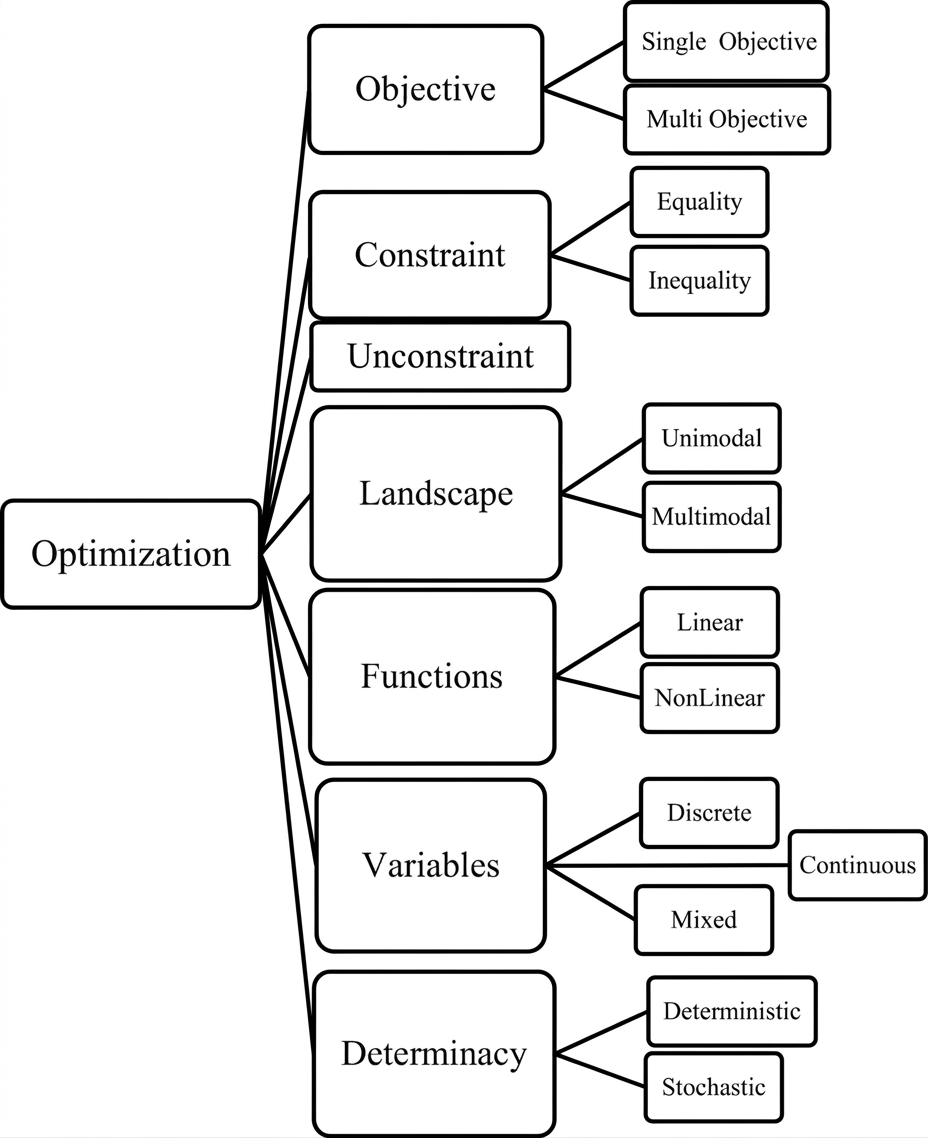
\includegraphics[width=0.48\textwidth]{./figuras/02_fundamentos_teoricos/problems_clasification.png}
    \caption{Taxonomía general de los problemas de optimización tomada de \cite{ahirwal2021swarm}.}
    \label{fig:problems_classification}
\end{figure}

Dentro de esta clasificación general, el presente trabajo se centra en problemas de \textbf{optimización continua monoobjetivo bajo restricciones de caja} (\textit{box constraints}). En este escenario, cada solución candidata deja de ser un elemento abstracto y se representa formalmente mediante un vector de variables reales \(\mathbf{x} = (x_1, x_2, \ldots, x_D)\), donde \(D\) denota la dimensión del problema y cada variable de decisión \(x_i\) toma valores dentro de un intervalo permitido.

De este modo, el marco matemático del problema de minimización considerado en esta investigación se plantea como:
\begin{equation}
    \min_{\mathbf{x} \in S} f(\mathbf{x}),
    \qquad
    S = \prod_{i=1}^{D} [l_i, u_i] \subset \mathbb{R}^{D}
\end{equation}
\noindent donde \(f:S \rightarrow \mathbb{R}\) es la función objetivo escalar, y \(l_i\) y \(u_i\) representan los límites inferior y superior que confinan el intervalo permitido para cada variable de decisión.

Adicionalmente, el alcance de este trabajo se restringe a entornos operativos de \textbf{caja negra} (\textit{black-box optimization}). Esto implica que los algoritmos de búsqueda carezcan de la capacidad de explotar información analítica y derivativa, debiendo guiar su comportamiento únicamente a través del valor escalar obtenido mediante la evaluación directa de soluciones.

En problemas no convexos o multimodales, la presencia de múltiples óptimos locales, mesetas y regiones irregulares dificulta el uso de métodos puramente locales o basados en gradiente. Por ello, resulta necesario recurrir a estrategias de búsqueda capaces de explorar el espacio de soluciones sin depender de información derivativa. Las principales familias de métodos utilizadas con este propósito se presentan en las secciones siguientes.


% Este escenario técnico adquiere su máxima complejidad cuando la superficie de búsqueda es \textbf{no convexa y multimodal}. En este tipo de paisajes, la aparición de múltiples óptimos locales, mesetas y regiones irregulares invalida los métodos de descenso tradicionales, exigiendo el uso de técnicas  ¡de optimización capaces de explorar eficientemente el espacio. Sin embargo, como se introdujo en el Capítulo~\ref{ref:introduccion}, la viabilidad de estos esquemas de búsqueda se ve muy comprometida en escenarios donde la evaluación de la función objetivo conlleva un alto coste computacional o se dispone de un presupuesto estrictamente restringido de evaluaciones. Es precisamente esta limitación fundamental la que restringe el uso de las principales técnicas de optimización y justifica, en última instancia, el desarrollo de las familias algorítmicas y los modelos de sustitución o \textit{surrogates} que se fundamentan en las siguientes secciones de este marco teórico.


% \subsubsection{Según la naturaleza de las variables}

% %% discreta vs continua

% La naturaleza de las variables de decisión determina en gran medida la estructura del problema de optimización. Cuando estas pueden tomar cualquier valor dentro de un intervalo, el problema es continuo. Cuando solo pueden asumir valores aislados o pertenecientes a conjuntos finitos, como ocurre en problemas de selección, asignación o permutación, el problema es discreto. Dentro de esta última categoría ocupan un lugar especialmente relevante los problemas \textbf{combinatorios}, en los que la solución implica seleccionar, asignar u ordenar elementos de entre un conjunto finito de posibilidades.

% Esta distinción resulta especialmente relevante porque influye tanto en la estructura del espacio de búsqueda como en los métodos que pueden emplearse para explorarlo. Mientras que los problemas continuos suelen admitir una modelización matemática más regular, los problemas discretos presentan con frecuencia una mayor complejidad combinatoria, lo que puede dificultar tanto su formulación como su resolución.

% \subsubsection{Según la linealidad del problema}

% % lineal vs no lineal

% La relación que mantienen las variables de decisión con la función objetivo y las restricciones no siempre presenta la misma complejidad. Cuando ambas pueden expresarse mediante relaciones lineales, el problema presenta una estructura más regular y, en general, más fácil de analizar y resolver. Cuando la función objetivo, alguna de las restricciones o ambas incorporan dependencias no lineales, la complejidad del problema aumenta y su resolución suele exigir estrategias más flexibles.

% \subsubsection{Según la convexidad del problema}

% %% convexos vs no convexos

% Una función es convexa si, para cualquier par de puntos en su dominio, el valor que toma sobre cualquier punto del segmento que los une es menor o igual que la combinación convexa de los valores de la función en dichos puntos \cite{boyd2004convex}. En el ámbito de la optimización, esta propiedad resulta especialmente relevante, ya que implica que todo óptimo local es también un óptimo global, lo que facilita la búsqueda de soluciones óptimas.

% Cuando esta condición no se cumple, el problema se considera no convexo. En estos casos, habituales en aplicaciones reales, la superficie de la función objetivo puede presentar múltiples óptimos locales, puntos de silla o regiones irregulares que dificultan el proceso de búsqueda y exige el uso de algoritmos con mayor capacidad de exploración, como las metaheurísticas.


% \subsubsection{Según el número de objetivos}

% En algunos problemas de optimización, la calidad de una solución viene determinada por una única función objetivo, lo que permite comparar directamente las alternativas mediante un solo valor. En otros casos intervienen múltiples objetivos \cite{hakanen2021multiobjective}, cuya optimización conjunta suele resultar más compleja, especialmente cuando entran en conflicto.

% En este contexto, la comparación entre soluciones deja de basarse en un orden total y se apoya habitualmente en el concepto de dominancia de Pareto. Una solución domina a otra si no es peor en ninguno de los objetivos y es mejor en al menos uno de ellos. Por ello, en optimización multiobjetivo no se busca normalmente una única solución óptima, sino un conjunto de soluciones no dominadas, denominado conjunto de Pareto, cuya imagen en el espacio de objetivos recibe el nombre de frente de Pareto \cite{deb2001multiobjective}.

% \subsubsection{Según las restricciones}

% %% con restricciones vs sin restricciones

% La presencia de restricciones \(\Omega\) delimita el conjunto de soluciones factibles y condiciona de forma directa la naturaleza del problema de optimización. En los problemas con restricciones, el objetivo consiste en optimizar la función \(f\) dentro del subconjunto de soluciones que satisfacen dichas condiciones, lo que suele requerir mecanismos específicos para garantizar la factibilidad y, en consecuencia, aumenta la dificultad de resolución. En los problemas sin restricciones, por el contrario, la búsqueda no está limitada por condiciones adicionales y se desarrolla sobre todo el espacio de búsqueda considerado.

\section{Estrategias de resolución: Metaheurísticas}

%% algoritmo aproximado frente a las exactas


%% Dinámicas de búsqueda: Exploración frente a explotación


%% Fenómenos críticos en computación evolutiva: Diversidad, estancamiento y convergencia prematura.

%% (Aquí se inserta el gráfico de Scopus para demostrar el auge del campo).


Debido a la relevancia práctica y teórica de los problemas de optimización en la ingeniería y las ciencias aplicadas, a lo largo del tiempo se ha desarrollado una amplia variedad de metodologías de resolución. Como se esquematiza en la Figura~\ref{fig:clasificacion_tecnicas_optimizacion}, estos enfoques abarcan desde procedimientos exactos, orientados a garantizar matemáticamente el hallazgo del óptimo global sacrificando la viabilidad temporal ante problemas complejos, hasta técnicas aproximadas.

Al trabajar sobre paisajes multimodales, no convexos y bajo condiciones de caja negra (\textit{black-box optimization}), el uso de métodos exactos resulta completamente inviable. Por ello, este trabajo se apoya en el marco operativo de las \textbf{metaheurísticas}, definidas como estrategias de aproximación de propósito general, a menudo no deterministas, que guían de forma eficiente a operadores de búsqueda abstractos con el fin de hallar soluciones de alta calidad en tiempos de cómputo razonables, renunciando a la garantía matemática de optimalidad global \cite{glover1986future, talbi2009metaheuristics, boussaid2013survey, marti2025fifty}.

\begin{figure}[H]
    \centering
    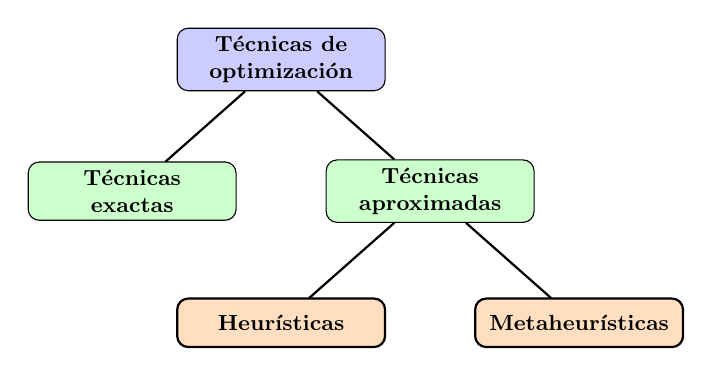
\begin{tikzpicture}[
            scale=0.88,
            transform shape,
            level distance=1.9cm,
            sibling distance=4.3cm,
            every node/.style={
                    rectangle,
                    rounded corners,
                    draw=black,
                    align=center,
                    minimum width=3.0cm,
                    minimum height=0.7cm,
                    font=\small
                },
            root/.style={
                    fill=blue!20,
                    font=\small\bfseries
                },
            levelone/.style={
                    fill=green!20,
                    font=\small\bfseries
                },
            leveltwo/.style={
                    fill=orange!25,
                    font=\small\bfseries
                },
            edge from parent/.style={
                    draw=black,
                    thick
                }
        ]

        \node[root] {Técnicas de\\optimización}
        child { node[levelone] {Técnicas\\exactas} }
        child { node[levelone] {Técnicas\\aproximadas}
                child { node[leveltwo] {Heurísticas} }
                child { node[leveltwo] {Metaheurísticas} }
            };

    \end{tikzpicture}
    \caption{Clasificación general de las técnicas para la resolución de problemas de optimización.}
    \label{fig:clasificacion_tecnicas_optimizacion}
\end{figure}

A diferencia de otras técnicas de aproximación, las metaheurísticas proporcionan un marco más general de búsqueda que puede adaptarse a distintas formulaciones mediante la incorporación de operadores, reglas o mecanismos dependientes del contexto \cite{talbi2009metaheuristics,gendreau2010handbook}. Su propósito no es recorrer exhaustivamente todas las soluciones posibles, sino explorar el espacio de búsqueda de manera eficiente, favoreciendo aquellas regiones que parecen prometedoras y reduciendo el esfuerzo invertido en zonas poco rentables.

Para justificar el impacto y el interés científico de estas metodologías, la Figura~\ref{fig:numero_papers_mh} ilustra la evolución bibliométrica del número de publicaciones indexadas en la base de datos Scopus bajo el término \textit{"metaheuristic"}. El crecimiento exponencial observado a lo largo de las últimas décadas evidencia la consolidación de este campo como una herramienta imprescindible para abordar problemas del mundo real donde los métodos tradicionales fallan.

\begin{figure}[H]
    \centering
    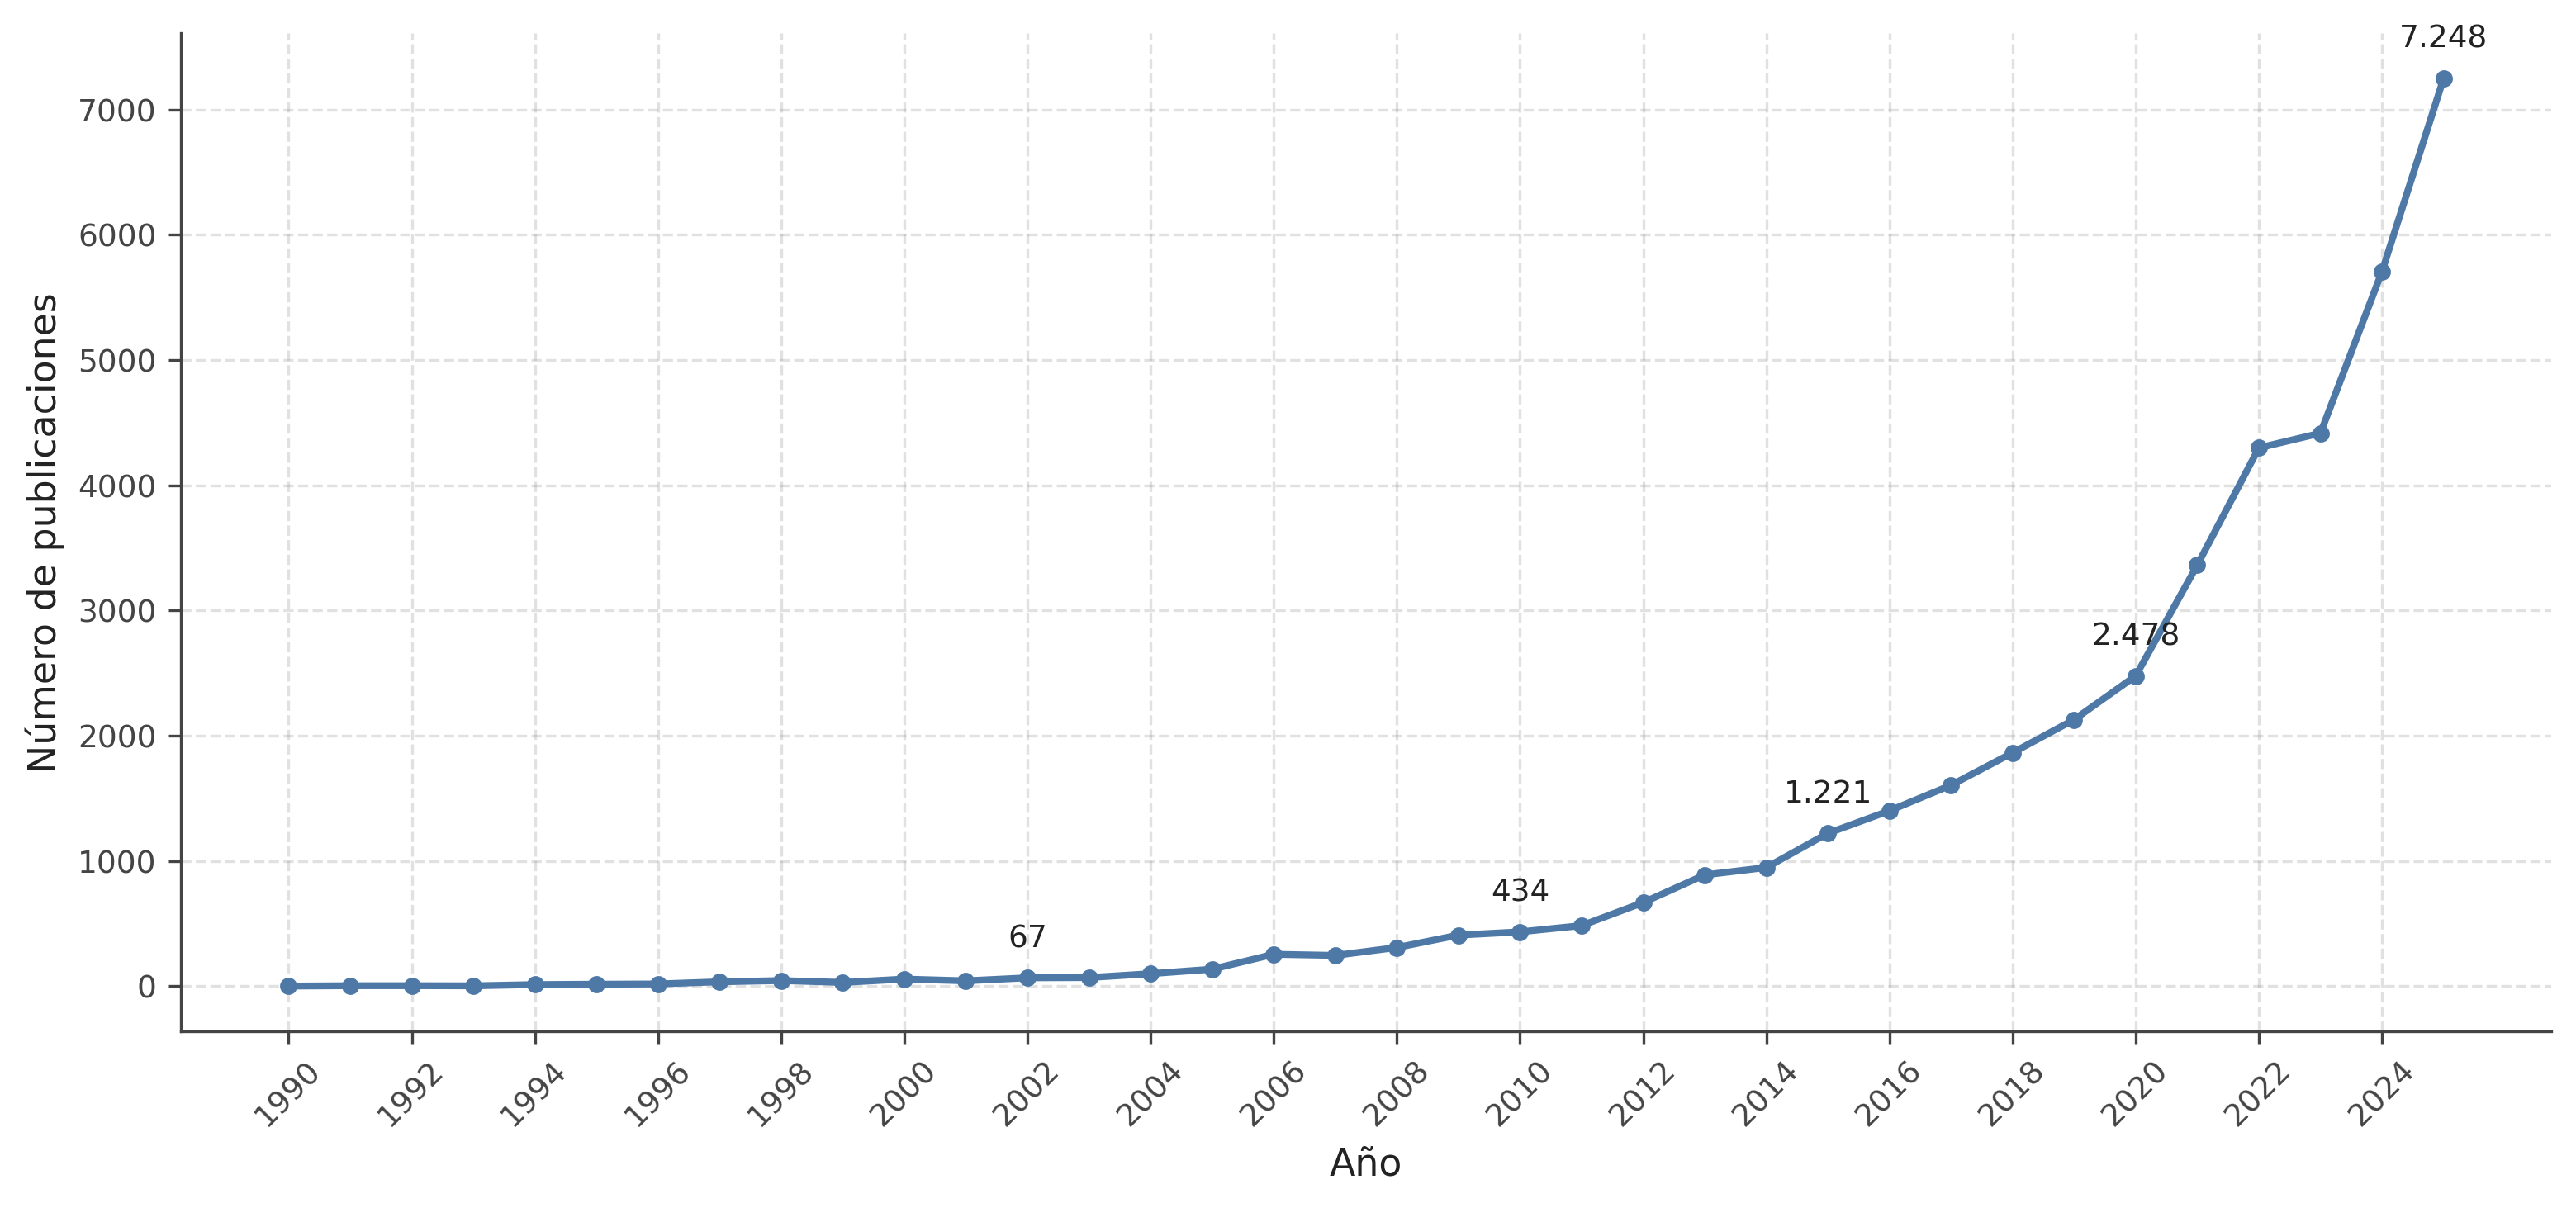
\includegraphics[width=1.0\textwidth]{./figuras/estado_del_arte/metaheuristicas_num_papers.png}
    \caption{Evolución anual del número de publicaciones sobre metaheurísticas en Scopus (1990--2025).}
    \label{fig:numero_papers_mh}
\end{figure}

Desde un punto de vista más abstracto, una metaheurística puede interpretarse como un esquema iterativo general parametrizable. Adaptando la formalización de \cite{luque2006resolucion}, denotamos el método como una tupla:

\begin{equation}
    \mathcal{M}=\langle \Theta,\Phi,\sigma,\mu,\lambda,\Xi,\tau\rangle
\end{equation}
\noindent donde $\Theta$ representa el conjunto de estructuras de trabajo, $\Phi$ el operador que genera nuevas candidatas, $\sigma$ la función que selecciona las estructuras que continúan en la siguiente iteración, $\mu$ y $\lambda$ el número de estructuras mantenidas y generadas, $\Xi$ el conjunto de variables de estado y $\tau$ el criterio de parada.

A partir de estas características generales, las metaheurísticas pueden organizarse según distintos criterios, entre ellos el tipo de estructura sobre la que articulan la búsqueda. Si bien se dividen taxonómicamente entre aquellas \textbf{basadas en trayectoria} ($\mu = 1$, orientadas a la explotación local mediante vecindarios) y las \textbf{basadas en poblaciones} ($\mu > 1$), este proyecto se enfoca exclusivamente en estas últimas.

\subsection{Dinámicas de búsqueda: Exploración, explotación y estancamiento}
\label{subsec:dinamicas_criticas}

Independientemente de la taxonomía o del diseño algorítmico de la metaheurística utilizada, el éxito en la resolución de problemas continuos complejos depende críticamente del balance dinámico entre dos conceptos totalmente opuestos presentes en sus operadores matemáticos:

\begin{definicion}
    La \textbf{exploración} amplía la búsqueda hacia regiones no visitadas del espacio de soluciones $S$ ayudando a evitar óptimos locales, mientras que la \textbf{explotación} intensifica la búsqueda alrededor de las mejores soluciones encontradas hasta el momento para su refinación.
\end{definicion}

\begin{figure}[H]
    \centering
    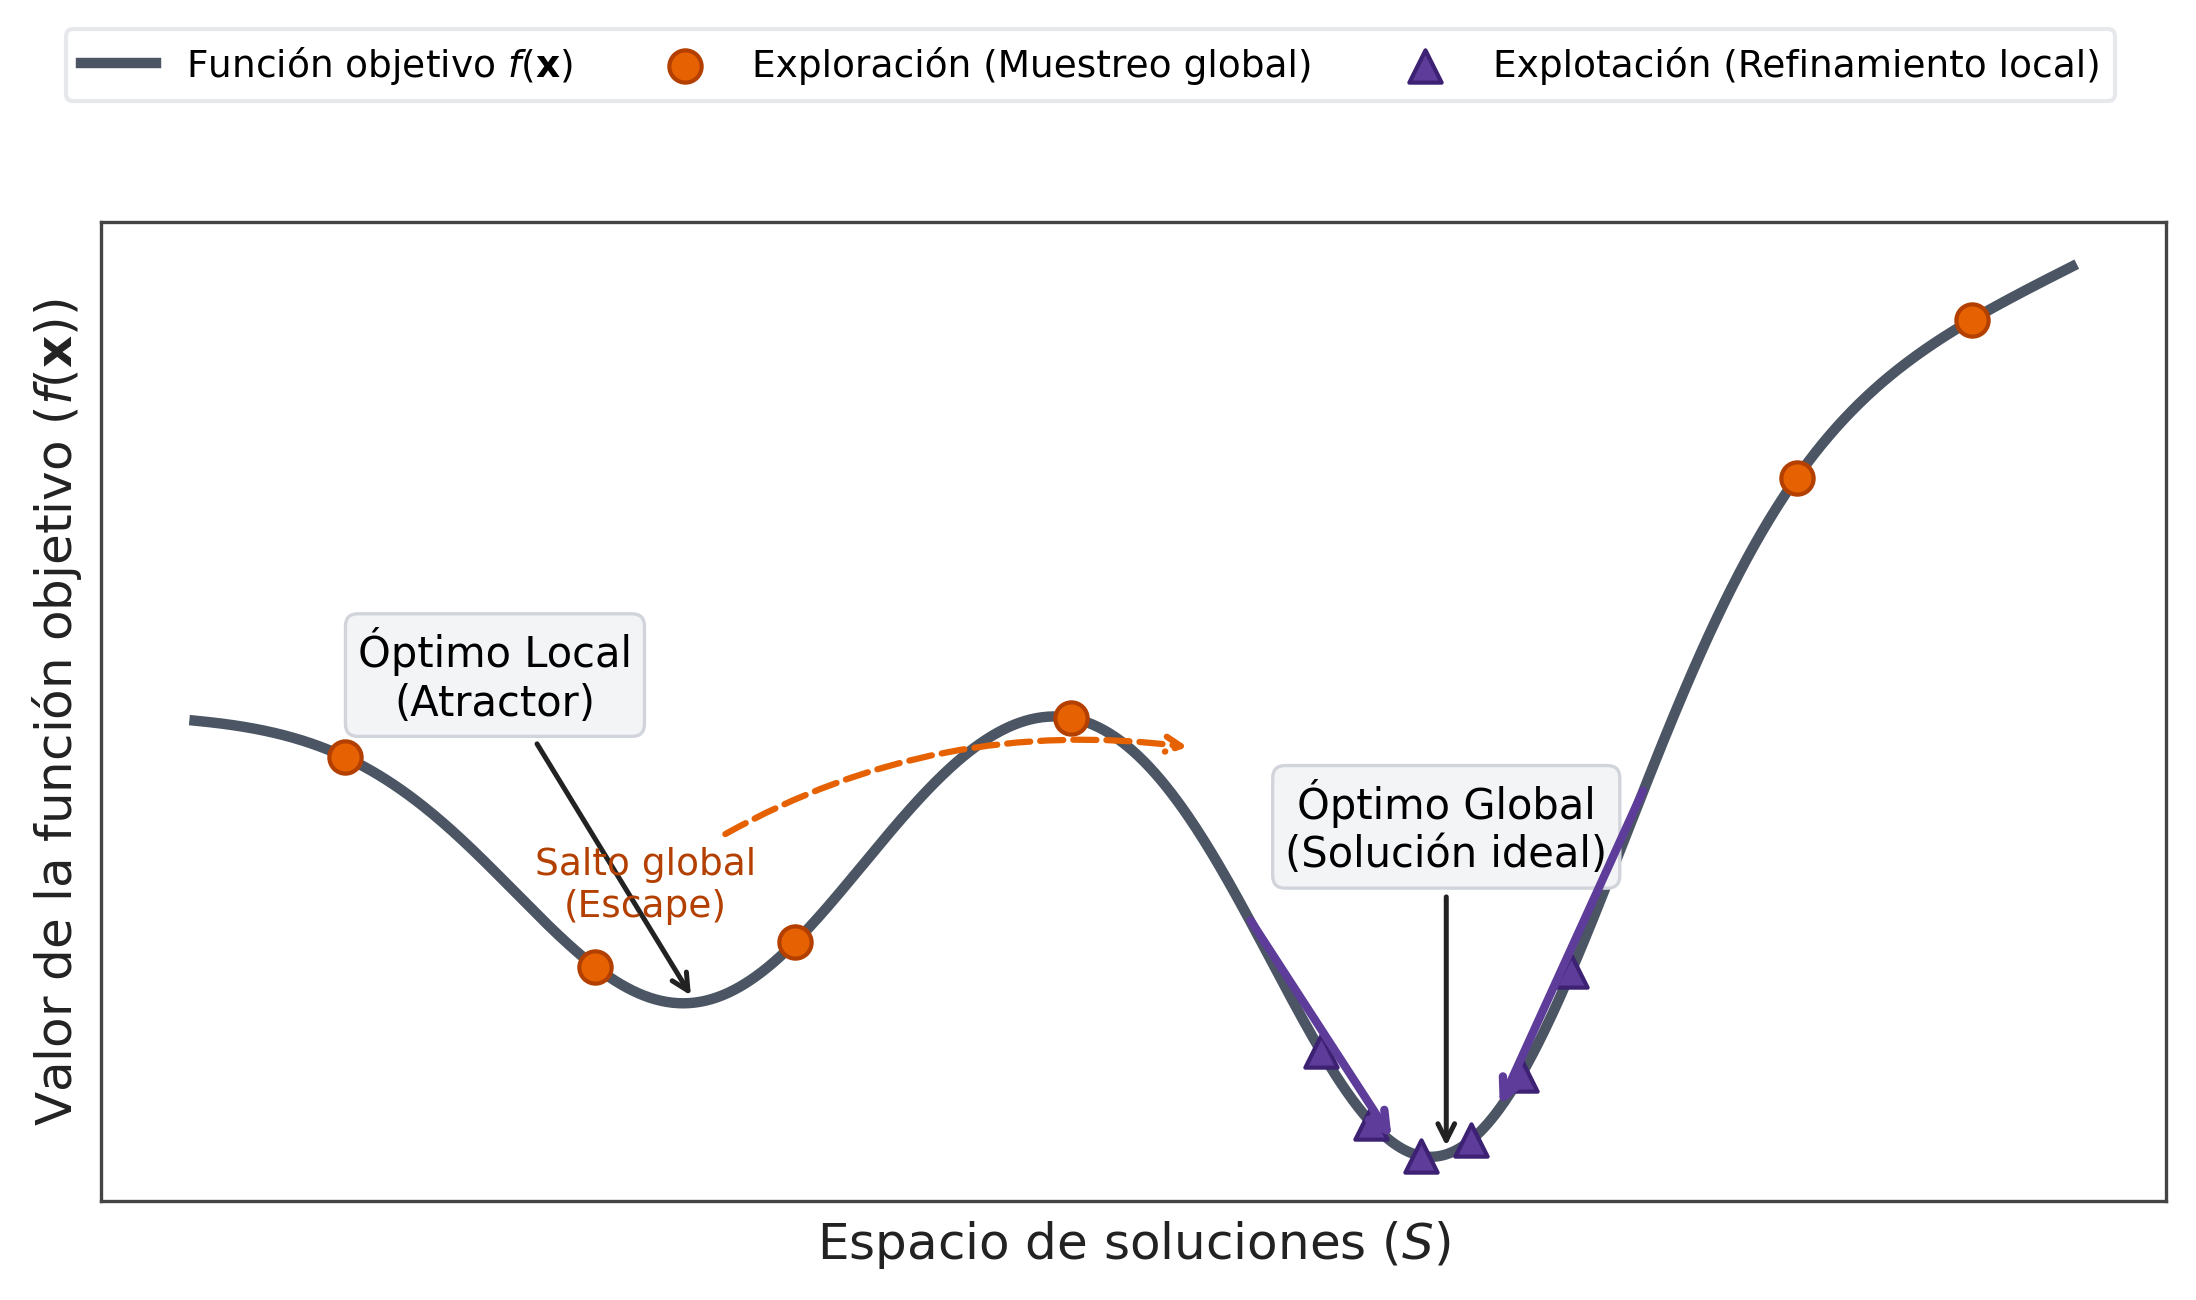
\includegraphics[width=0.8\textwidth]{figuras/02_fundamentos_teoricos/exploracion_explotacion_conceptual.png}
    \caption[Ilustración conceptual de la exploración y la explotación en un paisaje multimodal.]{Ilustración conceptual de la exploración y la explotación en un paisaje multimodal. La exploración distribuye muestras en distintas regiones del espacio de búsqueda, mientras que la explotación concentra la búsqueda alrededor de una zona prometedora para refinar la solución.}
    \label{fig:exploracion_explotacion}
\end{figure}

Durante el proceso iterativo de optimización, debe existir un equilibrio entre ambas fases. No obstante, también puede conducir a una intensificación excesiva o prematura bajo la cual la metaheurística sufre el fenómeno de la \textbf{convergencia prematura} \cite{pandey2014premature}. Este comportamiento ocurre cuando el algoritmo queda atrapado en un óptimo local, perdiendo la capacidad de escapar hacia otras zonas más prometedoras.

Como consecuencia directa de la convergencia prematura o de la caída en mesetas de gradiente nulo, se manifiesta el \textbf{estancamiento} \cite{squillero2016divergence}. Puede decirse que un algoritmo entra en dicha fase cuando, aun continuando con su ejecución, deja de producir mejoras significativas en la calidad de las soluciones durante un número prolongado de iteraciones o evaluaciones. Este comportamiento suele aparecer cuando los operadores quedan confinados en una región cuya explotación adicional apenas genera progreso. Si esta concentración ocurre demasiado pronto, la explotación pasa a dominar de forma excesiva sobre la exploración y el radio de búsqueda útil se colapsa antes de que el método haya revisado de forma suficientemente amplia otras zonas potencialmente prometedoras. En consecuencia, la convergencia prematura puede interpretarse como uno de los principales mecanismos que conducen al estancamiento en los procesos de optimización aproximada.

La mitigación del estancamiento motiva el diseño de estructuras más complejas, como las metaheurísticas poblacionales, así como la introducción de mecanismos de rescate dinámicos.

\subsection{Metaheurísticas basadas en poblaciones}
\label{subsec:mh_poblacion}

Las metaheurísticas basadas en poblaciones se caracterizan por trabajar simultáneamente con un conjunto de soluciones candidatas, a diferencia de los enfoques basados en trayectoria \cite{blum2003metaheuristics,boussaid2013survey}. Esta propiedad les permite mantener activas distintas regiones del espacio de búsqueda $S$ al mismo tiempo y aprovechar la información contenida en la distribución relativa de los individuos para orientar la dinámica del proceso de optimización \cite{talbi2009metaheuristics}.

En términos generales, su funcionamiento parte de una población inicial de soluciones por el espacio continuo $S$ que es evaluada, alterada mediante operadores estocásticos y actualizada aplicando cirerios de selección o reemplazo.

La principal ventaja de esta familia es su elevada capacidad exploratoria al muestrear distintas zonas del espacio de búsqueda e identificar regiones prometedoras, lo que reduce el riesgo de convergencia prematura. Sin embargo, esta ventaja conlleva un mayor coste computacional por ciclo, ya que en cada generación deben evaluarse multiples candidatos.

La propiedad fundamental que permite representar la dinámica de estas soluciones concurrentes y que determina la transición entre la exploración global y la explotación local es la \textbf{diversidad poblacional}:

\begin{definicion}
    La \textbf{diversidad poblacional} hace referencia a la variedad y heterogeneidad de las soluciones candidatas presentes en la población de una metaheurística. Mantener una diversidad adecuada es crucial para evitar el estancamiento y favorecer la exploración efectiva del espacio de búsqueda.
\end{definicion}

A medida que el algoritmo selecciona las regiones de mayor rendimiento, los individuos tienden a agruparse, contrayendo de forma natural la diversidad. No obstante, si esta pérdida de variabilidad ocurre de manera descontrolada, la población colapsa hacia la homogeneidad absoluta, volviendo a los individuos indistinguibles en el espacio continuo y dando lugar al estancamiento.

En el marco de este trabajo, este fenómeno es crítico. Al colapsar la diversidad, la heterogeneidad de las muestras recolectadas disminuye notablemente, provocando que los modelos de regresión y aprendizaje automático pierdan la capacidad estadística para entrenarse eficazmente y discriminar la calidad de nuevos candidatos \cite{omidvar2022review}.

Para mitigar este tipo de situaciones y evitar que el colapso de la diversidad limite tanto la búsqueda como la asistencia del modelo subrogado, pueden incorporarse \textbf{mecanismos de reinicio} encargados de reactivar la exploración cuando se detecta una ausencia prolongada de mejora \cite{fukunaga1998restart,lozano2008replacement}. El mecanismo concreto adoptado en este trabajo se describe en el Capítulo~\ref{chap:algo_tecnicas_ref}.

\subsection{Metaheurísticas evolutivas y operadores de la Computación Evolutiva}
\label{subsec:mh_evolutivas}

Dentro del paradigma de los métodos basados en poblaciones, las  \textbf{metaheurísticas evolutivas} constituyen una de las familias más robustas y ampliamente utilizadas en la literatura para la optimizacion continua  \cite{boussaid2013survey}.

Inspiradas en los mecanismos de adaptación y evolución observados en la naturaleza, estas técnicas hacen evolucionar un conjunto de soluciones candidatas llamado población a lo largo de ciclos iterativos denominados generaciones. Cada individuo se formaliza como un vector de variables reales $\mathbf{x} = (x_1, \dots, x_D) \in \mathbb{R}^D$, cuya adaptación cuantitativa al medio se califica a través de una función de aptitud o \textit{fitness} ($f(\mathbf{x})$) que mide la la calidad de la solución y guía el proceso de búsqueda \cite{talbi2009metaheuristics}.

La dinámica de búsqueda de una metaheurística evolutiva general, desde su inicialización hasta el cumplimiento de los criterios de parada, está determinado por la aplicación de cuatro operadores universales \cite{luke2013essentials}:

\begin{enumerate}
    \item \textbf{Selección de progenitores (o de padres):} Mecanismo encargado de elegir qué individuos de la población actual tendrán prioridad para reproducirse, asegurando que las soluciones con mejor rendimiento (\textit{fitness} más óptimo) transmitan su información a las siguientes iteraciones.
    \item \textbf{Operadores de variación (Cruce y Mutación):} Constituyen el motor de generación de diversidad y exploración del algoritmo:
          \begin{itemize}
              \item \textit{Cruce:} Operador que toma dos o más soluciones seleccionadas como padres e intercambia o combina sus componentes vectoriales para dar lugar a nuevos individuos descendientes (\textit{offspring}). Su papel es explotar y comunicar regiones prometedoras ya descubiertas.
              \item \textit{Mutación:} Operador unario que altera aleatoriamente uno o varios componentes de un vector descendiente. Su papel es puramente exploratorio, introduciendo diversidad para evitar el estancamiento en óptimos locales.
          \end{itemize}
    \item \textbf{Evaluación de soluciones:} Fase en la que se calcula el valor de $f(\mathbf{x})$ para cada nuevo descendiente generado. Si el cálculo de $f(\mathbf{x})$ exige una coste computacional elevado, el coste de evaluar poblaciones enteras de forma recurrente vuelve inviable la optimización evolutiva.
    \item \textbf{Reemplazo (Selección de supervivientes):} Mecanismo encargado de decidir qué elementos, entre la población original y el conjunto de nuevos descendientes, conformarán la población que sobrevive y pasa a la siguiente generación.
\end{enumerate}

De esta manera, la dinámica de un algoritmo evolutivo puede resumirse en el Algoritmo~\ref{alg:ea_general}.

\begin{algorithm}[H]
    \caption{Esquema general de un algoritmo evolutivo}
    \label{alg:ea_general}
    \begin{algorithmic}[1]
        \State $P \gets \textsc{GenerarPoblacionInicial}()$
        \State $\textsc{Evaluar}(P)$
        \While{no se cumpla el criterio de parada}
        \State $P' \gets \textsc{SeleccionarPadres}(P)$
        \State $P' \gets \textsc{Cruzar}(P')$
        \State $P' \gets \textsc{Mutar}(P')$
        \State $\textsc{Evaluar}(P')$
        \State $P \gets \textsc{SeleccionarNuevaPoblacion}(P, P')$
        \EndWhile
        \State \Return mejor solución encontrada
    \end{algorithmic}
\end{algorithm}

Dentro de esta familia se incluyen distintas líneas metodológicas, entre ellas los algoritmos genéticos o las estrategias evolutivas, que comparten el enfoque poblacional y evolutivo, aunque difieren en la forma en que generan nueva descendencia y en los operadores que emplean.


% %% tecnicas de optimizacion

% \begin{figure}[htbp]
%     \centering
%     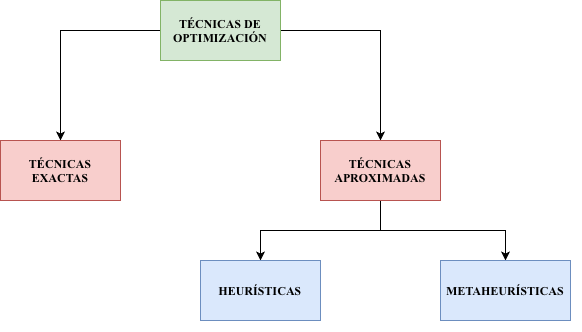
\includegraphics[width=0.85\textwidth]{./figuras/clasificacion_tecnicas_optimizacion/clasificacion_tecnicas_optimizacion.drawio.png}
%     \caption{Clasificación general de las técnicas de optimización.}
%     \label{fig:optimization_methods}
% \end{figure}
%% tecnicas exactas: garantia del optimo

% \subsection{Técnicas exactas}

% Las técnicas exactas constituyen aquellos métodos de optimización que, bajo una formulación adecuada del problema y con un presupuesto de cómputo suficiente, garantizan la obtención de la solución óptima. En este grupo se incluyen, por ejemplo, la programación lineal, la programación entera, la programación dinámica y otros procedimientos matemáticos basados en propiedades estructurales del problema.

% Su principal ventaja reside en que proporcionan garantías teóricas sobre la optimalidad de la solución obtenida. Sin embargo, esta característica suele ir acompañada de una fuerte dependencia de la formulación del problema y de un crecimiento significativo del coste computacional a medida que aumenta la complejidad del espacio de búsqueda. Por ello, cuando el problema es grande, no convexo o carece de una estructura explotable de forma directa, estas técnicas pueden resultar poco adecuadas o incluso inviables en escenarios reales.


% %% tecnicas aproximadas: sacrificio de la garantia del optimo por tiempo

% \subsection{Técnicas aproximadas}

% Aunque las técnicas exactas componen el marco de referencia desde el punto de vista teórico, en la práctica numerosos problemas de optimización deben abordarse mediante métodos aproximados capaces de proporcionar soluciones de calidad aceptable dentro de un presupuesto computacional razonable. Estas técnicas no aseguran, en general, la obtención del óptimo global, pero permiten afrontar problemas de gran escala o elevada complejidad en los que los procedimientos exactos resultan inviables por su coste o por la ausencia de una estructura suficientemente explotable \cite{boussaid2013survey}.

% El interés por este tipo de enfoques se debe a su capacidad para equilibrar calidad de solución y eficiencia temporal. Dentro de esta categoría se distinguen, de forma general, las \textbf{heurísticas} y las \textbf{metaheurísticas}, que constituyen dos de los marcos más utilizados en la optimización moderna. Aunque ambas persiguen soluciones de buena calidad en tiempos razonables, difieren en su alcance, grado de generalidad y capacidad para adaptarse a distintos problemas de optimización.

% %% heuristicas

% \subsubsection{Heurísticas}

% Generalmente, el término \textit{heurística} se utiliza para designar estrategias prácticas de resolución de problemas que permiten orientar la búsqueda de soluciones cuando no resulta viable, o no es necesario, aplicar un procedimiento exacto o exhaustivo \cite{handbookheuristics2018}. En optimización, esta idea se traduce en métodos capaces de explotar de forma eficiente la estructura del problema para obtener soluciones de calidad aceptable.

% \begin{definicion}
%     Las heurísticas son procedimientos de búsqueda orientados a obtener soluciones de buena calidad en un tiempo de cómputo reducido, sin garantizar la optimalidad de la solución obtenida.
% \end{definicion}

% Su interés radica en que permiten abordar problemas complejos en los que la resolución exacta resulta poco práctica debido al elevado coste computacional o al tamaño del espacio de búsqueda \cite{springer2024heuristics}.

% Según la forma en que generan o refinan las soluciones, las heurísticas suelen agruparse en distintas familias \cite{franca1999adaptive}. \textbf{Las heurísticas constructivas} construyen una solución desde cero, incorporando decisiones de manera progresiva hasta completar una solución factible. \textbf{Las heurísticas de mejora} parten de una solución inicial y la refinan mediante modificaciones locales orientadas a incrementar su calidad. \textbf{Las heurísticas híbridas} combinan ambos enfoques o integran estrategias adicionales de búsqueda con el objetivo de aprovechar las ventajas de cada una de ellas \cite{moreira2013hybrid}.

% %% metaheuristicas

% % - son métodos no exactos y, por lo general, no deterministas
% % - guían el proceso de búsqueda
% % - realizan una exploración eficiente del espacio de búsqueda
% % - tienen una estructura básica predefinida
% % - pueden incorporar heurísticos específicos dependientes del problema
% % - usan mecanismos para evitar regiones poco prometedoras
% % - son iterativos y disponen de criterios de parada
% % - persiguen soluciones cuasi óptimas

% % - idea: la armonización entre exploración y explotación como uno de los rasgos clave de la eficiencia de una metaheurística

% \subsubsection{Metaheurísticas}

% Las metaheurísticas constituyen una familia de métodos de optimización no exactos, diseñados para obtener soluciones de alta calidad en tiempos de cómputo razonables, especialmente en problemas complejos para los que los métodos exactos resultan inviables desde un punto de vista práctico \cite{glover1986future,talbi2009metaheuristics,boussaid2013survey}. En términos generales, se trata de procedimientos, a menudo no deterministas, concebidos para guiar de forma eficiente el proceso de búsqueda a través del espacio de soluciones \cite{talbi2009metaheuristics,luke2013essentials,marti2025fifty}.

% A diferencia de las heurísticas específicas de problema, las metaheurísticas proporcionan un marco más general de búsqueda que puede adaptarse a distintas formulaciones mediante la incorporación de operadores, reglas o mecanismos dependientes del contexto \cite{talbi2009metaheuristics,gendreau2010handbook}. Su propósito no es recorrer exhaustivamente todas las soluciones posibles, sino explorar el espacio de búsqueda de manera eficiente, favoreciendo aquellas regiones que parecen prometedoras y reduciendo el esfuerzo invertido en zonas poco rentables.

% En la mayoría de los casos, su funcionamiento se apoya en una estructura básica predefinida sobre la que se construyen mecanismos de generación, evaluación y actualización de soluciones. Este proceso se repite hasta que se satisface algún criterio de parada, como un número máximo de iteraciones, un límite temporal o una condición de convergencia \cite{luke2013essentials}. Como resultado, las metaheurísticas persiguen soluciones de calidad suficientemente alta para numerosos problemas reales, aunque sin garantizar optimalidad global \cite{glover1986future,talbi2009metaheuristics,boussaid2013survey}.

% Uno de los principios fundamentales en el diseño de metaheurísticas es el equilibrio entre exploración y explotación \cite{talbi2009metaheuristics,luke2013essentials,boussaid2013survey}. La exploración permite recorrer distintas regiones del espacio de búsqueda y reducir el riesgo de convergencia prematura, mientras que la explotación concentra el esfuerzo computacional en refinar aquellas zonas que ya han mostrado soluciones prometedoras. La capacidad para armonizar ambos comportamientos constituye uno de los elementos que más influye en la eficacia y robustez de estos métodos.

% Desde un punto de vista más abstracto, una metaheurística puede interpretarse como un esquema iterativo general compuesto por un conjunto de soluciones o estructuras de trabajo, un operador de generación de nuevas candidatas, un mecanismo de selección o reemplazo, un conjunto de variables de estado y un criterio de parada. Esta formalización, adaptada de \cite{luque2006resolucion}, permite describir bajo un mismo marco metaheurísticas de naturaleza muy distinta:
% \[
%     \mathcal{M}=\langle \Theta,\Phi,\sigma,\mu,\lambda,\Xi,\tau\rangle,
% \]
% donde \(\Theta\) es el conjunto de estructuras con las que trabaja el método, \(\Phi\) el operador que genera nuevas candidatas, \(\sigma\) la función que selecciona las estructuras que continúan en la siguiente iteración, \(\mu\) y \(\lambda\) el número de estructuras mantenidas y generadas, \(\Xi\) el conjunto de variables de estado del algoritmo y \(\tau\) el criterio de parada.

% A partir de estas características generales, las metaheurísticas pueden organizarse según distintos criterios, entre ellos el tipo de estructura sobre la que articulan la búsqueda. Esta distinción permite introducir las principales familias de métodos que se describen a continuación.

% \begin{figure}[H]
%     \centering
%     \begin{tikzpicture}[
%         node distance=0.8cm and 2.3cm,
%         every node/.style={font=\scriptsize},
%         box/.style={
%                 draw,
%                 rounded corners,
%                 align=center,
%                 minimum height=0.6cm,
%                 minimum width=2.4cm
%             },
%         rootbox/.style={
%                 box,
%                 fill=gray!15,
%                 text width=2.6cm
%             },
%         childbox/.style={
%                 box,
%                 fill=blue!8,
%                 text width=2.3cm
%             },
%         subclass/.style={
%                 box,
%                 fill=gray!3,
%                 text width=2.1cm
%             },
%         arrow/.style={
%         -{Latex[length=2mm]},
%         thick
%         }
%         ]

%         \node[rootbox] (root) {Metaheurísticas};
%         \node[childbox, below left=1.1cm and 1.5cm of root] (pop) {Basadas en\\población};
%         \node[childbox, below right=1.1cm and 0.8cm of root] (tray) {Basadas en\\trayectoria};

%         \matrix (subpops) [below=2.0cm of pop, column sep=1.8cm, row sep=0cm] {
%             \node[subclass] (enjambre) {Basadas en\\inteligencia de enjambre}; &
%             \node[subclass] (hibridas) {Híbridas};                             &
%             \node[subclass] (evolutivas) {Evolutivas};                           \\
%         };

%         \draw[arrow] (root) -- (pop);
%         \draw[arrow] (root) -- (tray);

%         \draw[arrow] (pop) -- (enjambre);
%         \draw[arrow] (pop) -- (hibridas);
%         \draw[arrow] (pop) -- (evolutivas);

%     \end{tikzpicture}
%     \caption{Clasificación general de las metaheurísticas según el tipo de estructura de búsqueda.}
%     \label{fig:clasificacion_metaheuristicas}
% \end{figure}

% \paragraph{Metaheurísticas basadas en trayectoria}

% Las metaheurísticas basadas en trayectoria se caracterizan por trabajar, en cada iteración, sobre una única solución actual o sobre un número muy reducido de soluciones estrechamente relacionadas \cite{blum2003metaheuristics,boussaid2013survey}. A partir de esa solución, el algoritmo genera nuevas candidatas mediante movimientos definidos sobre su vecindario, de modo que la búsqueda va construyendo una trayectoria a través del espacio de soluciones \cite{talbi2009metaheuristics}.

% En muchos casos, estos métodos se consideran extensiones de los procedimientos clásicos de búsqueda local. Mientras que una búsqueda local simple suele detenerse al alcanzar un óptimo local, las metaheurísticas basadas en trayectoria incorporan mecanismos adicionales para escapar de esas regiones y continuar explorando otras zonas del espacio de búsqueda \cite{gendreau2010handbook,luke2013essentials}. Entre dichos mecanismos pueden encontrarse la aceptación controlada de soluciones peores, el uso de memoria o la modificación del vecindario.

% Su principal ventaja reside en que permiten intensificar la búsqueda de manera muy eficiente alrededor de soluciones prometedoras. Sin embargo, esta misma concentración sobre una única trayectoria puede reducir la diversidad explorada y aumentar el riesgo de convergencia prematura si no se incorporan mecanismos adecuados de diversificación \cite{blum2003metaheuristics,boussaid2013survey}. Dentro de esta familia se incluyen metaheurísticas como \textit{Simulated Annealing} \cite{kirkpatrick1983optimization,vanderbilt1984monte,pedamallu2008investigating}, \textit{Tabu Search} \cite{glover1989tabu,rachid2000tabu} o \textit{Variable Neighborhood Search}. Desde la formalización abstracta introducida anteriormente, este comportamiento se corresponde típicamente con el uso de una única estructura activa por iteración, de modo que \(\mu = 1\), y con la generación de un número reducido de nuevas estructuras, por lo que \(\lambda\) suele ser pequeño.

% \paragraph{Metaheurísticas basadas en poblaciones}

% Las metaheurísticas basadas en poblaciones se caracterizan por trabajar simultáneamente con un conjunto de soluciones candidatas, en lugar de guiar la búsqueda a partir de una única solución actual \cite{blum2003metaheuristics,boussaid2013survey}. Esta característica les permite mantener activas distintas regiones del espacio de búsqueda al mismo tiempo y aprovechar la información contenida en la distribución relativa de los individuos para orientar la evolución del proceso de optimización \cite{talbi2009metaheuristics,luke2013essentials}.

% En términos generales, su funcionamiento parte de una población inicial de soluciones, a partir de la cual se generan nuevas candidatas utilizando la información disponible en los individuos ya presentes. Posteriormente, dichas soluciones se evalúan y la población se actualiza según algún criterio de selección o reemplazo \cite{talbi2009metaheuristics,boussaid2013survey}. El intercambio de información entre soluciones puede modelarse de distintas maneras, como la recombinación entre individuos, el uso de diferencias entre soluciones o la atracción hacia posiciones prometedoras.

% Una de las principales ventajas de esta familia es su elevada capacidad exploratoria. Al mantener múltiples soluciones simultáneamente, las metaheurísticas poblacionales pueden muestrear distintas zonas del espacio de búsqueda, identificar regiones prometedoras y reducir el riesgo de convergencia prematura asociado a la concentración temprana en una sola trayectoria \cite{blum2003metaheuristics,boussaid2013survey,omidvar2022review}. No obstante, esta ventaja suele ir acompañada de un mayor coste computacional por iteración, ya que en cada ciclo deben evaluarse varias soluciones candidatas. Esta observación resulta especialmente relevante en problemas con funciones objetivo costosas, donde el uso de grandes poblaciones puede hacer necesario recurrir a estrategias de aceleración, paralelización o modelado \textit{surrogate} \cite{omidvar2022review}.

% Desde la formalización abstracta introducida anteriormente, las metaheurísticas basadas en poblaciones se caracterizan por operar con varias estructuras activas en cada iteración, por lo que \(\mu > 1\). Del mismo modo, el número de nuevas estructuras generadas en cada ciclo también suele ser superior al de los métodos basados en trayectoria, de manera que \(\lambda > 1\).

% \subparagraph{Metaheurísticas poblacionales basadas en inteligencia de enjambre}

% Las metaheurísticas basadas en inteligencia de enjambre modelan comportamientos colectivos descentralizados, en los que múltiples agentes interactúan entre sí y con el entorno para orientar la búsqueda. En esta familia se sitúan, entre otros, \textit{Particle Swarm Optimization} \cite{kennedy1995pso} o \textit{Ant Colony Optimization} \cite{socha2008aco}.

% \subparagraph{Metaheurísticas poblacionales híbridas}

% Las metaheurísticas híbridas poblacionales combinan mecanismos de búsqueda poblacional con procedimientos adicionales de intensificación, como búsqueda local o estrategias meméticas, con el objetivo de combinar exploración global y refinamiento local \cite{lozano2004memetic,ong2004metalamarckian,renders1996hybrid,hart1994adaptive}. Dentro de este panorama también pueden situarse enfoques basados en modelado probabilístico, como los \textit{Estimation of Distribution Algorithms} \cite{ahn2008eda}.

% \subparagraph{Metaheurísticas poblacionales evolutivas}

% Los algoritmos evolutivos (EA) constituyen una familia de metaheurísticas poblacionales inspiradas en los mecanismos de adaptación y evolución observados en la naturaleza. De forma general, operan sobre una población de individuos que representan soluciones candidatas al problema. A lo largo del proceso de búsqueda, dicha población evoluciona mediante operadores de selección, variación y reemplazo \cite{holland1975adaptation,mitchell1998introduction,reeves2003genetic,affenzeller2009genetic}. Cada individuo recibe una valoración cuantitativa a través de una función de aptitud o \textit{fitness}, que mide la calidad de la solución representada y guía el proceso de búsqueda.

% De forma abstracta, la dinámica de un algoritmo evolutivo puede resumirse en el Algoritmo~\ref{alg:ea_general}. En primer lugar, se genera una población inicial y se evalúa su calidad. A continuación, mientras no se satisfaga el criterio de parada, se seleccionan progenitores, se aplican operadores de recombinación y mutación para generar descendencia, se evalúan los nuevos individuos y se actualiza la población mediante algún mecanismo de reemplazo. El proceso iterativo finaliza devolviendo la mejor solución encontrada.

% \begin{algorithm}[H]
%     \caption{Esquema general de un algoritmo evolutivo}
%     \label{alg:ea_general}
%     \begin{algorithmic}[1]
%         \State $P \gets \textsc{GenerarPoblacionInicial}()$
%         \State $\textsc{Evaluar}(P)$
%         \While{no se cumpla el criterio de parada}
%         \State $P' \gets \textsc{SeleccionarPadres}(P)$
%         \State $P' \gets \textsc{Recombinar}(P')$
%         \State $P' \gets \textsc{Mutar}(P')$
%         \State $\textsc{Evaluar}(P')$
%         \State $P \gets \textsc{SeleccionarNuevaPoblacion}(P, P')$
%         \EndWhile
%         \State \Return mejor solución encontrada
%     \end{algorithmic}
% \end{algorithm}

% Dentro de esta familia se incluyen distintas líneas metodológicas, entre ellas los algoritmos genéticos, las estrategias evolutivas y métodos posteriores como \textit{Differential Evolution}, que comparten el enfoque poblacional y evolutivo, aunque difieren en la forma en que generan nueva descendencia y en los operadores que emplean.


\section{Aprendizaje Automático Orientado a la Regresión}
\label{sec:aprendizaje_automatico}

Si bien el campo de la optimización metaheurística se centra en el diseño de estrategias eficientes para explorar espacios de búsqueda complejos, la computación moderna ofrece otro gran paradigma para abordar problemas de caja negra: el \textbf{Aprendizaje Automático} (\textit{Machine Learning}). Aunque históricamente ambas disciplinas han evolucionado como comunidades científicas independientes y con objetivos diferenciados, su convergencia metodológica proporciona hoy en día un marco robusto para la resolución de problemas de alta complejidad computacional.

A diferencia de los enfoques algorítmicos tradicionales, el Aprendizaje Automático es un subcampo de la inteligencia artificial que no pretende codificar instrucciones explícitas para resolver una tarea, sino que dota a los sistemas informáticos de la capacidad de aprender y extraer patrones de los datos sin necesidad de ser programados explícitamente \cite{mitchell1997machine, bishop2006pattern}.


\subsection{Formalización de los conjuntos de datos en el aprendizaje}

Para comprender cómo un sistema computacional extrae conocimiento, es necesario formalizar matemáticamente los componentes informacionales que se requieren. Desde una perspectiva formal, la información disponible se estructura a partir de un conjunto global de observaciones realizadas a partir del conjunto de datos denotado como:

\begin{equation}
    \mathcal{D} = \{(\mathbf{x}_1, y_1), (\mathbf{x}_2, y_2), \dots, (\mathbf{x}_N, y_N)\} = \{(\mathbf{x}_i, y_i)\}_{i=1}^N
\end{equation}

\noindent donde $\mathbf{x}_i \in \mathbb{R}^D$ representa el vector de características (que en el contexto de este proyecto se corresponderá con las variables de decisión de un candidato) e $y_i$ constituye la etiqueta o respuesta real asociada (la evaluación real del problema).

Con el fin de garantizar un aprendizaje correcto y evitar estimaciones sesgadas u optimistas basadas en la mera memorización de datos (\textbf{sobreajuste}), la metodología del Aprendizaje Automático exige la partición estricta de $\mathcal{D}$ en subconjuntos disjuntos y especializados con propósitos bien definidos \cite{bishop2006pattern}:

\begin{itemize}
    \item \textbf{Conjunto de entrenamiento ($\mathcal{D}_{\text{train}}$):} Subconjunto de datos utilizado para ajustar los parámetros del modelo mediante el algoritmo de aprendizaje.
    \item \textbf{Conjunto de validación ($\mathcal{D}_{\text{val}}$):} Subconjunto independiente que no interviene en el entrenamiento que se emplea para evaluar el rendimiento del modelo durante el proceso de desarrollo y para ajustar sus hiperparámetros. Su objetivo es proporcionar una estimación no sesgada del rendimiento del modelo y ayudar a prevenir el sobreajuste, guiando la selección del modelo y su configuración final.
\end{itemize}

\begin{figure}[htbp]
    \centering
    \begin{tikzpicture}[
            node distance = 0.8cm and 1.5cm,
            block/.style = {rectangle, draw, fill=blue!10, minimum width=3.5cm, minimum height=1.2cm, align=center, rounded corners, font=\small},
            trainblock/.style = {rectangle, draw, fill=green!10, minimum width=4cm, minimum height=1.2cm, align=center, rounded corners, font=\small},
            valblock/.style = {rectangle, draw, fill=orange!10, minimum width=4cm, minimum height=1.2cm, align=center, rounded corners, font=\small}
        ]
        % Nodo principal
        \node [block] (dataset) {Conjunto Global $\mathcal{D}$\\ (Histórico de Evaluaciones)};

        % Nodos de partición (Entrenamiento y Validación)
        \node [trainblock, above right=of dataset] (train) {Conjunto de Entrenamiento $\mathcal{D}_{\text{train}}$\\ ($\approx 70-80\%$)};
        \node [valblock, below right=of dataset] (val) {Conjunto de Validación $\mathcal{D}_{\text{val}}$\\ ($\approx 20-30\%$)};

        % Flechas de flujo
        \draw [->, thick] (dataset.east) -- ++(0.5,0) |- (train.west);
        \draw [->, thick] (dataset.east) -- ++(0.5,0) |- (val.west);

        % Indicador de exclusión mutiva (Conjuntos disjuntos)
        \path (train) -- node[font=\scriptsize\color{red!80!black}, fill=white, inner sep=2pt] (disjoint) {$\mathcal{D}_{\text{train}} \cap \mathcal{D}_{\text{val}} = \emptyset$} (val);
        \draw [dashed, red!50] (train.south) -- (val.north);

    \end{tikzpicture}
    \caption{Esquema metodológico de la partición del conjunto global $\mathcal{D}$ en los subconjuntos disjuntos de entrenamiento ($\mathcal{D}_{\text{train}}$) y validación ($\mathcal{D}_{\text{val}}$).}
    \label{fig:particion_datos}
\end{figure}

\subsection{Paradigmas de aprendizaje y el enfoque supervisado}

Una vez definidos estos bloques fundamentales de información, la naturaleza y la disponibilidad de $\mathcal{D}_{\text{train}}$ y $\mathcal{D}_{\text{val}}$ permiten delimitar formalmente los cuatro grandes paradigmas del Aprendizaje Automático \cite{russell2020artificial}:

\begin{itemize}
    \item \textbf{Aprendizaje supervisado:} El conjunto de entrenamiento con el que se alimenta al algoritmo incluye las soluciones deseadas, denominadas etiquetas. El objetivo del algoritmo es aprender un mapeo generalizable que asocie nuevas entradas con sus salidas correspondientes.
    \item \textbf{Aprendizaje semi-supervisado:} Etiquetar los datos suele llevar mucho tiempo y ser costoso, por lo que el conjunto de entrenamiento tiene a muchos casos sin etiquetar y pocos casos etiquetados.
    \item \textbf{Aprendizaje no supervisado:} El algoritmo recibe un conjunto de datos sin etiquetas ni respuestas asociadas, siendo su objetivo descubrir patrones dentro del espacio de características.
    \item \textbf{Aprendizaje por refuerzo:} A diferencia de los enfoques anteriores, el algoritmo no aprende a partir de un conjunto de datos estático con etiquetas, sino que interactúa con un entorno dinámico y aprende una política de decisión que maximiza una recompensa acumulada.
\end{itemize}

Este trabajo se apoya estrictamente en el marco del \textbf{aprendizaje supervisado}.

%% evaluar si aqui hay que explicar los distainos problemas regrsion clasifiacjon
\subsection{El problema de la regresión continua}

%% esta bien definida la regresion o no

Dentro del aprendizaje supervisado, la naturaleza de la variable de salida \(y\) determina el tipo de problema a resolver. Cuando la respuesta pertenece a un conjunto discreto o categórico, el escenario se define como un problema de \textit{clasificación}. Por el contrario, cuando la variable de salida es numérica y continua, \(y \in \mathbb{R}\), se trata de un problema de \textbf{regresión}.

\begin{figure}[H]
    \centering
    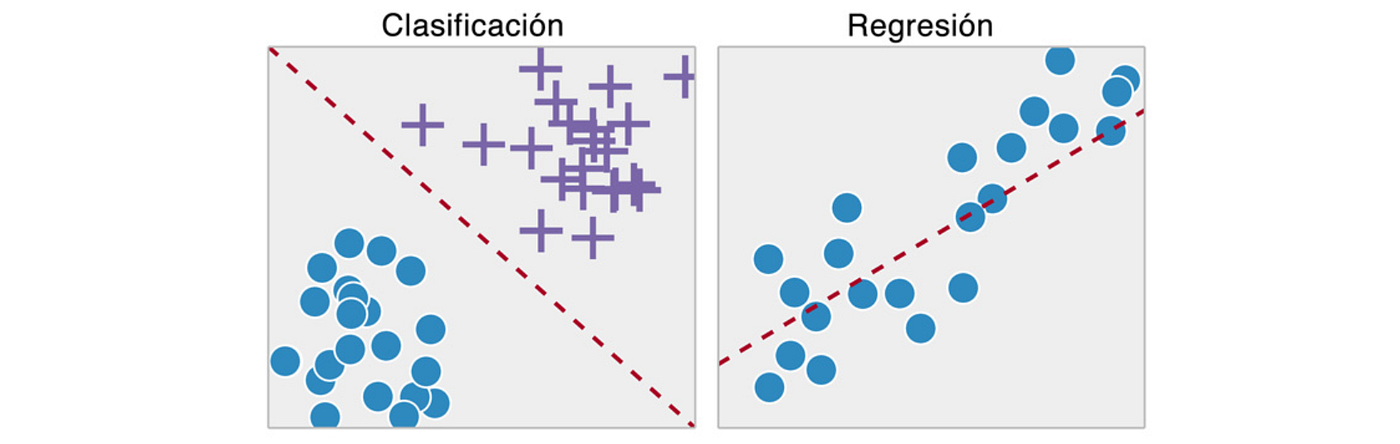
\includegraphics[width=0.7\textwidth]{figuras/02_fundamentos_teoricos/diferencia_clasificacion_regresion.png}
    \caption{Ilustración comparativa entre problemas de clasificación y regresión.}
    \label{fig:regresion_vs_clasificacion}
\end{figure}

Este trabajo se enmarca en el ámbito de la regresión, ya que en optimización continua cada vector de decisión \(\mathbf{x}_i\) tiene asociado un valor real de calidad dado por la función objetivo \(f(\mathbf{x}_i)\). El propósito del modelo supervisado consiste, por tanto, en aprender una aproximación de la relación entre las soluciones candidatas y sus valores de \textit{fitness} a partir de las muestras recolectadas en el conjunto \(\mathcal{D}_{\text{train}}\).

% En este contexto, los modelos de aprendizaje automático actúan como aproximadores predictivos basados en datos. A partir de un conjunto finito de evaluaciones previas, tratan de estimar el valor de la función objetivo en nuevas soluciones candidatas para que la función objetivo real únicamente evalúe las mejores, proporcionando un sustituto computacionalmente más ligero que la evaluación directa del problema original.

\subsection{Taxonomía general de los modelos de regresión}

Para abordar la aproximación predictiva de la función de aptitud a partir de las muestras de $\mathcal{D}_{\text{train}}$, la literatura científica ofrece una amplia diversidad de enfoques algorítmicos en función de cómo modelan la relación entre las variables de entrada (en este contexto, variables de decisión) y el espacio de salida.

A continuación, se describen las cinco grandes filosofías de modelado predictivo para tareas de regresión continua, sentando las bases teóricas de los paradigmas que se compararán en este trabajo.

\subsubsection{Modelos lineales}

Esta familia constituye el pilar histórico de la estadística descriptiva y el aprendizaje supervisado. Su principio operativo asume que la variable de salida se puede aproximar mediante una combinación lineal ponderada de las variables de entrada, donde cada característica es ponderada por un coeficiente numérico que el algoritmo debe optimizar.


% Aunque su capacidad para capturar interacciones no lineales de alta complejidad o paisajes de \textit{fitness} extremadamente rugosos es intrínsecamente limitada (bajo sesgo y alta varianza en escenarios complejos), su velocidad de cómputo es prácticamente instantánea y ofrecen una interpretabilidad absoluta. En el contexto de los modelos subrogados, su uso es altamente valioso como línea base descriptiva (\textit{baseline}) y para aproximar tendencias globales en regiones locales del espacio de búsqueda.

Aunque su capacidad para capturar interacciones no lineales complejas es limitada, su velocidad de cómputo es prácticamente instantánea, no requieren configuraciones complejas y ofrecen una interpretabilidad matemática directa sobre la contribución global de cada variable en el modelo predictivo. Dentro de esta familia se encuentran, por ejemplo, la regresión lineal ordinaria o las variantes regularizadas como Ridge, LASSO o Elastic Net, las cuales introducen penalizaciones matemáticas para controlar la varianza y la complejidad del modelo.

\subsubsection{Modelos basados en árboles y ensambles}

Estos enfoques sustituyen la búsqueda de una función matemática global por una estrategia de particionado recursivo del espacio de características. El modelo base segmenta el dominio de manera jerárquica mediante umbrales lógicos, aislando las muestras en regiones disjuntas denominadas hojas, donde la predicción se establece como el valor promedio de los datos locales de entrenamiento (como se ilustra en la Figura \ref{fig:arbol_decision_regresion}).

\begin{figure}[H]
    \centering
    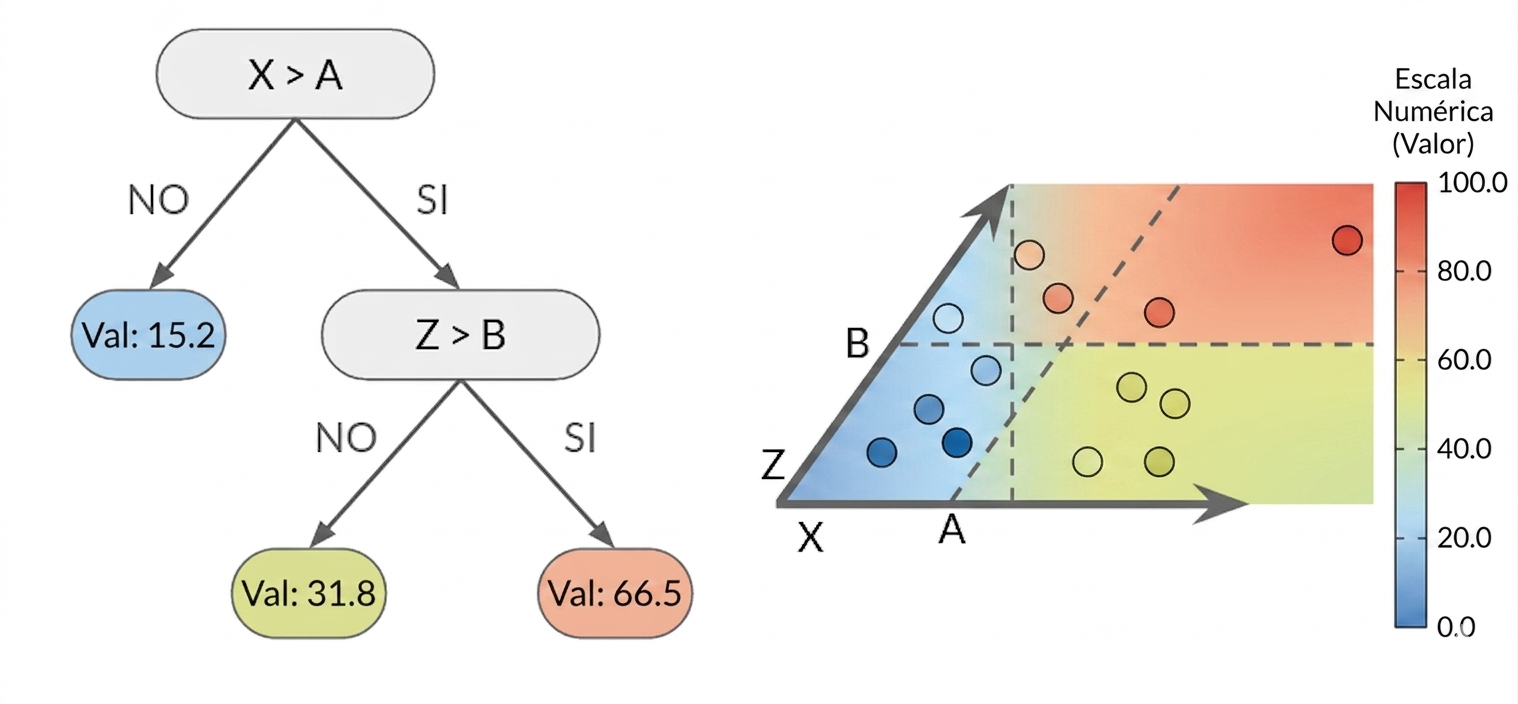
\includegraphics[width=0.7\textwidth]{figuras/02_fundamentos_teoricos/arbol_decision_regresion.png}
    \caption[Ejemplo conceptual de un árbol de decisión aplicado a regresión.]{Ejemplo conceptual de un árbol de decisión aplicado a regresión, donde el espacio de entrada se divide mediante reglas sucesivas hasta asignar una predicción numérica en cada región terminal.}
    \label{fig:arbol_decision_regresion}
\end{figure}

Para suavizar las predicciones escalonadas características de un único árbol de regresión y mitigar su tendencia al sobreajuste, las técnicas modernas recurren a los métodos de ensamble. Estos enfoques combinan las predicciones de múltiples árboles mediante estrategias de agregación en paralelo a través de remuestreo (\textit{bagging}, como en \textit{Random Forest}) o mediante la corrección secuencial y aditiva de los errores residuales de los estimadores previos (\textit{boosting}, como en los algoritmos de \textit{Gradient Boosting} o XGBoost), adaptándose con gran precisión y robustez a las discontinuidades del espacio.

\subsubsection{Modelos basados en vectores de soporte y aprendizaje estadístico}

%% deberiamos citar que es eso del aprendizaje estadistico

Nacidos de la teoría del aprendizaje estadístico, estos modelos abordan la regresión desde una perspectiva geométrica y de optimización convexa.

Su principio básico consiste en buscar una función aproximadora con buena capacidad de generalización, evitando ajustar de forma exacta todas las observaciones del conjunto de entrenamiento. Esta idea se formaliza mediante un margen de tolerancia alrededor de la función predicha. Los errores que quedan dentro de dicho margen no se penalizan, mientras que solo las muestras que lo exceden influyen de forma efectiva en el ajuste del modelo. Estas muestras relevantes reciben el nombre de \textbf{vectores de soporte}, ya que determinan la forma final de la función aprendida.

Una característica relevante de esta familia es el uso de funciones \textit{kernel}, que permiten trabajar de forma implícita en espacios de mayor dimensión sin construir explícitamente dicha transformación, siendo la técnica de Regresión por Vectores de Soporte (\textit{Support Vector Regression}, SVR) el máximo exponente de esta filosofía predictiva en problemas de salida continua.

\subsubsection{Métodos de vecindad y funciones de base}

Esta familia predictiva se basa en la similitud y localidad de los datos: aquellas observaciones que se encuentren a una distancia espacial reducida dentro del dominio de entrada deben presentar valores de salida similares.

Estos métodos computan la predicción de una nueva instancia calculando una interpolación o promedio ponderado de los puntos conocidos más cercanos de $\mathcal{D}_{\text{train}}$, donde la influencia de cada muestra disminuye a medida que aumenta su distancia geométrica respecto al punto a predecir. En esta categoría pueden situarse métodos como \(k\)-Nearest Neighbors para regresión, aproximadores basados en funciones de base radial (RBF) o técnicas de interpolación local.

\subsubsection{Redes neuronales artificiales (\textit{Deep Learning})}

Inspiradas en las dinámicas de transmisión de información de los sistemas biológicos, las redes neuronales estructuran el aprendizaje mediante el encadenamiento jerárquico y masivo de capas de unidades elementales de procesamiento (neuronas artificiales), tal y como se detalla en la Figura \ref{fig:redes_neuronales}, capaces de capturar patrones y relaciones altamente complejas y no lineales.

\begin{figure}[H]
    \centering
    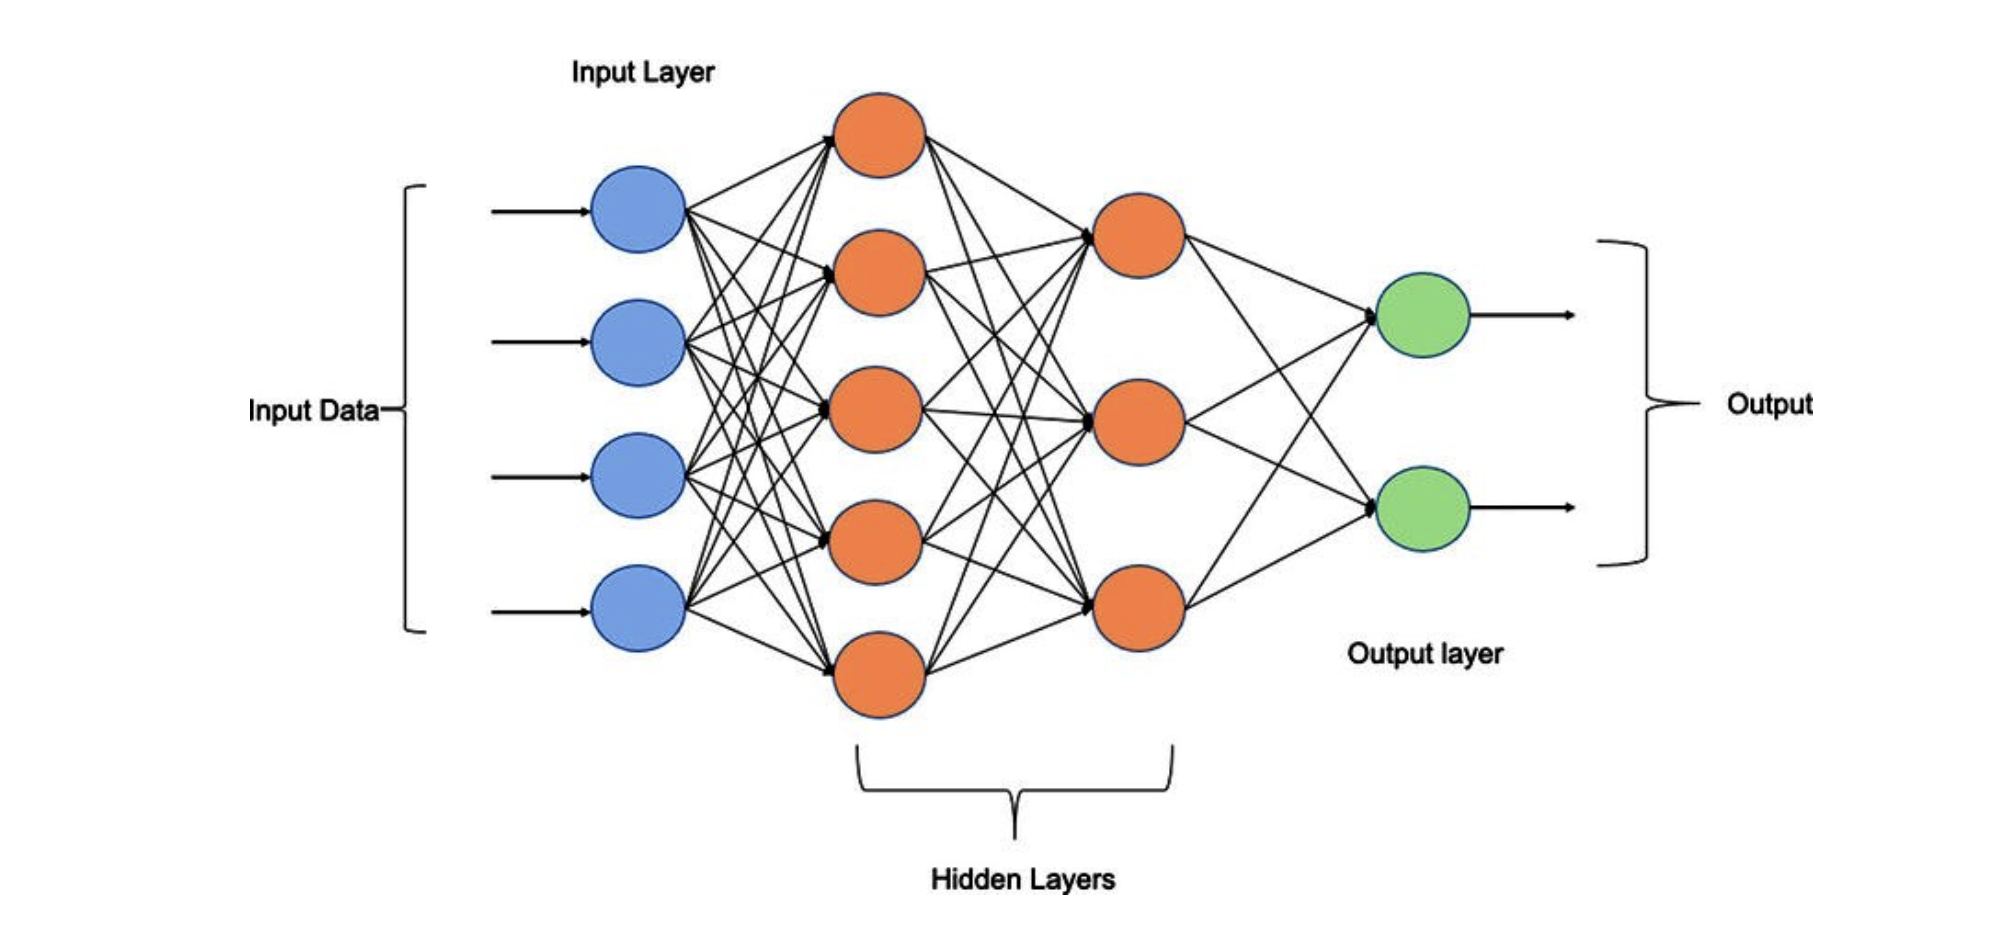
\includegraphics[width=0.65\textwidth]{figuras/02_fundamentos_teoricos/redes_neuronales.png}
    \caption{Esquema conceptual de una red neuronal artificial organizada en capas de entrada, capas ocultas y capa de salida.}
    \label{fig:redes_neuronales}
\end{figure}

Este entrelazado sucesivo de transformaciones les capacita para inducir automáticamente representaciones abstractas de los datos de entrada a lo largo de sus capas, lo que les permite modelar interacciones continuas de extrema complejidad matemática a costa de una mayor demanda de recursos computacionales para su ajuste. El Perceptrón Multicapa (\textit{Multilayer Perceptron}, MLP) asenta las bases clásicas de esta familia en tareas de regresión, asumiendo como contrapartida una alta demanda de recursos computacionales y un volumen de datos elevado para su correcto ajuste.

%% Fundamentos del aprendizaje supervisado y la regresión técnica
%% Taxonomía general de modelos basados en datos: Modelos lineales, basados en árboles (ensamblados) y redes neuronales (Deep Learning) a nivel conceptual.

%% definir los distintos tipos de aprendizaje, destacandno el supervisoda, que es donde se encuentra la regresion.

\section{Técnicas Subrogadas}
\label{sec:tecnicas_subrogadas}

En problemas de optimización continua, una de las principales limitaciones prácticas aparece cuando la evaluación de la función objetivo requiere un coste computacional elevado. Esta situación es habitual en problemas de caja negra basados en simulaciones, modelos físicos, análisis numéricos complejos o procesos experimentales, donde cada evaluación puede implicar un tiempo de cálculo elevado o incluso prohibitivo \cite{queipo2005surrogate,forrester2009recent}. En estos escenarios, una metaheurística poblacional puede necesitar miles de evaluaciones para explorar adecuadamente el espacio de búsqueda, haciendo que el coste total del proceso resulte difícilmente asumible.

Las \textbf{técnicas subrogadas} surgen como una estrategia para reducir este coste. Su idea fundamental consiste en construir un modelo aproximado de la función objetivo a partir de un conjunto limitado de soluciones ya evaluadas. Dicho modelo, denominado modelo subrogado, permite estimar de forma rápida la calidad de nuevas soluciones candidatas sin recurrir siempre a la evaluación real del problema \cite{queipo2005surrogate,forrester2009recent,jin2011surrogate}.

Sea \(f:\mathcal{X}\rightarrow\mathbb{R}\) una función objetivo costosa de evaluar, un modelo subrogado es una aproximación construida a partir de un conjunto finito de muestras evaluadas
\[
    \mathcal{D}=\{(\mathbf{x}_i,f(\mathbf{x}_i))\}_{i=1}^{n},
\]
cuyo propósito es proporcionar información útil sobre el comportamiento de \(f\) con un coste computacional significativamente menor que el de la evaluación directa. Habitualmente, esta información se materializa en una función predictiva \(\hat{f}:\mathcal{X}\rightarrow\mathbb{R}\), aunque también puede adoptar otras formas abstractas orientadas a comparar, clasificar o priorizar soluciones.

Desde esta perspectiva, los modelos subrogados no constituyen una familia independiente de algoritmos de optimización, sino una forma específica de utilizar modelos predictivos dentro del proceso de búsqueda.

Históricamente, esta función ha sido desempeñada tanto por aproximaciones estadísticas y matemáticas clásicas, como \textit{Kriging}, procesos gaussianos o expansiones de caos polinómico (\textit{Polynomial Chaos Expansion}, PCE), como por modelos modernos de aprendizaje automático. Estos últimos pueden actuar como subrogados cuando se entrenan con pares \((\mathbf{x}, f(\mathbf{x}))\) y se emplean, bajo un enfoque de regresión supervisada, para aproximar la relación entre una solución candidata y su valor de \textit{fitness}. Por tanto, la diferencia no reside únicamente en el modelo empleado, sino en el papel que este desempeña: sustituir, apoyar o guiar parcialmente las evaluaciones reales de la función objetivo.

Aunque los modelos subrogados suelen plantearse como aproximaciones directas de la función objetivo, su utilidad en optimización no se limita necesariamente a predecir con total precisión el valor numérico de \(f\). En muchos casos, resulta suficiente con que proporcionen información útil para orientar la búsqueda, por ejemplo preservando el orden relativo entre soluciones, discriminando entre candidatas prometedoras y no prometedoras o apoyando decisiones de selección sin necesidad de reproducir exactamente la función original. Esta distinción permite clasificar las técnicas subrogadas en función del tipo de información que intentan predecir como modelos orientados al \textbf{fitness absoluto} o modelos orientados al \textbf{fitness relativo} \cite{tong2021surrogate}.

\subsection{Clasificación según el tipo de predicción}
\label{subsec:clasificacion_surrogates_prediccion}

La clasificación propuesta en la Figura \ref{fig:clasificacion_sgs} resulta especialmente útil en el contexto de la optimización evolutiva, ya que separa los modelos en función de la información que proporcionan al algoritmo de búsqueda.

\begin{figure}[H]
    \centering
    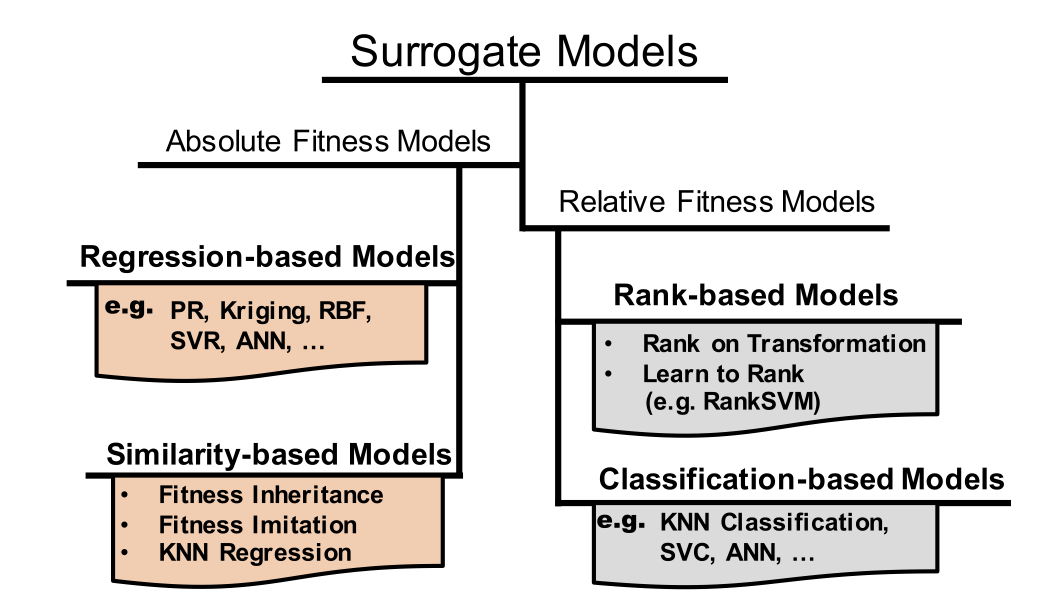
\includegraphics[width=0.7\textwidth]{./figuras/clasificacion_surrogates/clasificacion_sgs.png}
    \caption{Clasificación de las técnicas subrogadas según el tipo de predicción, adaptada de \cite{tong2021surrogate}.}
    \label{fig:clasificacion_sgs}
\end{figure}

Los modelos de \textbf{fitness absoluto} intentan estimar el valor numérico exacto de la función objetivo para una solución candidata. Bajo este enfoque, el subrogado se utiliza como una función aproximada \(\hat{f}\) capaz de asignar una predicción escalar a cada punto del espacio de búsqueda. Esta formulación coincide con el uso más clásico de los modelos subrogados, ya que permite sustituir una evaluación costosa por una predicción directa del \textit{fitness}. Dentro de esta categoría se sitúan, entre otros, los modelos basados en regresión y los métodos basados en similitud local, que estiman la calidad de una solución a partir de su relación con muestras previamente evaluadas.

Por el contrario, los modelos de \textbf{fitness relativo} no buscan reproducir el valor real de la función objetivo, sino inferir relaciones comparativas entre soluciones. En este caso, el subrogado se utiliza para estimar qué candidato es preferible, qué soluciones deberían ocupar posiciones superiores en un ranking o qué individuos pertenecen a una región prometedora del espacio de búsqueda. Este enfoque resulta especialmente relevante cuando el objetivo del optimizador no es conocer la magnitud cuantitativa de cada solución o este es difícil de estimar, sino tomar decisiones de selección, reemplazo o priorización entre candidatos, tareas que a menudo resultan menos exigentes estadísticamente que ajustar con precisión sus valores absolutos \cite{yuxue2024effective}.

Esta segunda perspectiva conecta directamente con el planteamiento experimental del presente trabajo. En una metaheurística poblacional, muchas decisiones estratégicas, como la selección de progenitores o el reemplazo de individuos, dependen del orden relativo entre soluciones más que de la magnitud exacta de sus valores de \textit{fitness}. Por ello, en el estudio de modelos orientados al fitness relativo, es de especial relevancia evaluar si el subrogado es capaz de conservar correctamente dicha estructura ordinal a lo largo de las distintas etapas de la búsqueda, lo que justifica teóricamente el uso de métricas basadas en la correlación de rangos para valorar la fidelidad cualitativa de las aproximaciones.

\subsection{Clasificación según el modo de integración}

No obstante, la utilización de técnicas subrogadas también plantea limitaciones importantes. Si el modelo aproximado no está correctamente ajustado, puede inducir al algoritmo de optimización a explorar regiones poco prometedoras del espacio, establecer un orden incorrecto entre soluciones o descartar prematuramente candidatas óptimas. Asimismo, muchos modelos presentan dificultades para generalizar fuera de las zonas en las que han sido entrenados, lo que restringe su utilidad en espacios de búsqueda amplios o con una estructura altamente no lineal \cite{forrester2009recent,bhosekar2018advances}. Por ello, la eficacia final de estos métodos depende tanto de la calidad de los datos empleados para su entrenamiento como del modo en que se integran dentro del proceso de optimización.

En función de dicha integración, la literatura distingue distintos esquemas de uso. En estrategias \textit{offline}, el modelo se entrena previamente con un conjunto de datos disponible y posteriormente se evalúa su capacidad para reproducir o anticipar el comportamiento de la función objetivo. En estrategias \textit{online}, en cambio, el subrogado se actualiza durante la propia ejecución de la metaheurística, incorporando nuevas evaluaciones reales conforme avanza la búsqueda. Dentro de esta segunda familia se sitúan enfoques como \textit{Sequential Model-Based Optimization} (SMBO), donde el modelo y la función real interactúan de forma iterativa. Por otro lado, esquemas como \textit{Predict-then-Optimise} (PtO) plantean una separación más clara entre la fase de entrenamiento del modelo y la posterior optimización sobre la aproximación construida \cite{bliek2022sustainableSBO}.

\subsubsection{Sequential Model-Based Optimization (SMBO)}
\label{subsec:smbo}

El enfoque \textit{Sequential Model-Based Optimization} se caracteriza por la alternancia iterativa entre el subrogado y la función objetivo costosa. En una primera fase se evalúa un conjunto inicial de soluciones reales con el fin de construir un conjunto de entrenamiento. A partir de esos datos se ajusta un modelo sustituto, que posteriormente se utiliza para proponer o priorizar nuevas soluciones prometedoras. Dichas soluciones son evaluadas de nuevo sobre la función real y la información obtenida se incorpora al conjunto disponible para actualizar el subrogado.

La característica distintiva de este esquema es que el modelo no sustituye definitivamente a la función objetivo, sino que se refina progresivamente a medida que avanza la búsqueda. Por ello, este tipo de integración suele asociarse a estrategias \textit{online}, en las que el subrogado actúa como un mecanismo auxiliar que orienta la exploración y reduce el número de evaluaciones reales necesarias.

\begin{figure}[H]
    \centering
    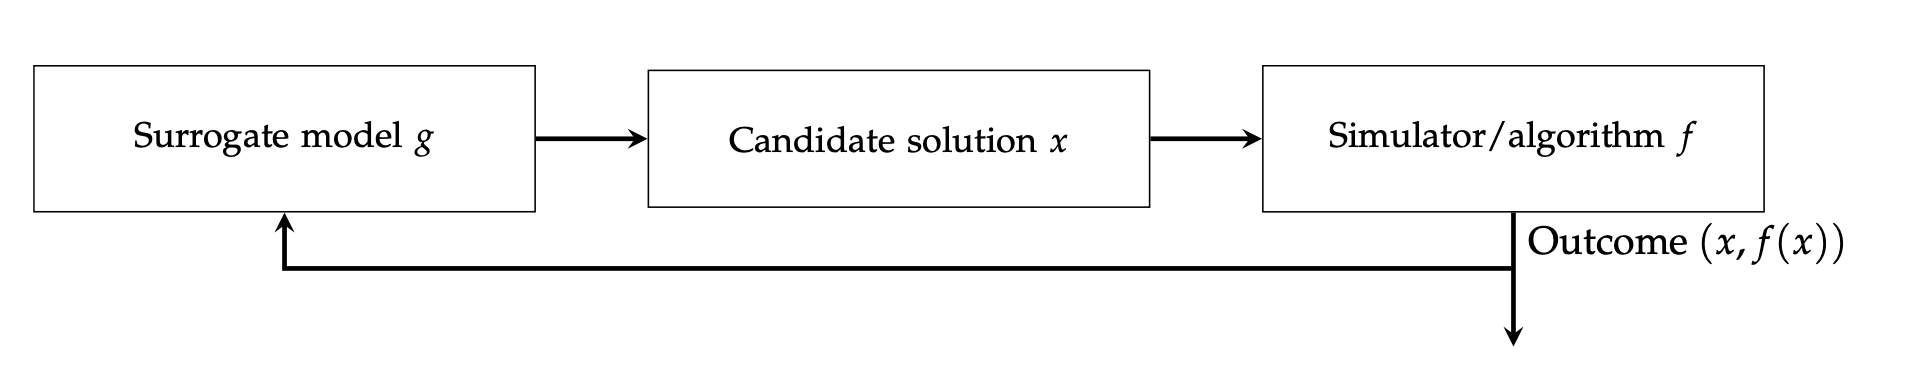
\includegraphics[width=0.95\textwidth]{./figuras/clasificacion_surrogates/smbo.png}
    \caption{Framework simplificado de un algoritmo SMBO típico obtenido de \cite{bliek2022sustainableSBO}.}
    \label{fig:smbo}
\end{figure}

La Figura~\ref{fig:smbo} muestra este ciclo de realimentación continua entre subrogado, optimización y evaluación real, donde cada nueva evaluación contribuye a mejorar la calidad del modelo.

\subsubsection{Predict-then-Optimise (PtO)}

En el enfoque \textit{Predict-then-Optimise}, el subrogado se entrena previamente a partir de un conjunto de muestras evaluadas sobre la función real y, una vez construido, pasa a utilizarse como aproximación sobre la que opera el algoritmo de búsqueda. En este caso, la fase de construcción del modelo y la fase de optimización quedan más separadas que en SMBO, ya que el modelo no se actualiza necesariamente de forma iterativa durante la búsqueda.

La principal ventaja de este esquema es que, tras el entrenamiento inicial, la optimización puede desarrollarse con un coste de evaluación mucho menor. Sin embargo, la calidad del resultado depende de la fidelidad del subrogado, ya que cualquier sesgo o error acumulado en la aproximación puede trasladarse directamente a las decisiones del optimizador. Por este motivo, PtO suele asociarse a estrategias \textit{offline} o a escenarios donde se desea estudiar previamente la capacidad del modelo para reproducir el comportamiento de la función objetivo.

\begin{figure}[H]
    \centering
    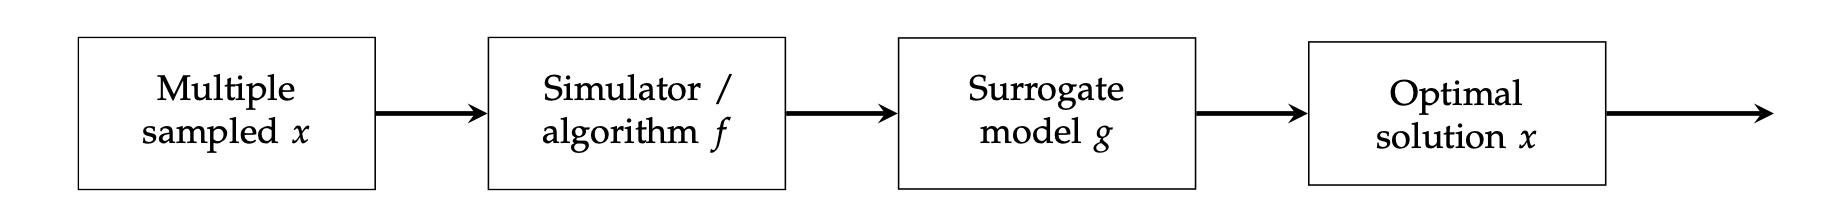
\includegraphics[width=1.00\textwidth]{./figuras/clasificacion_surrogates/pto.png}
    \caption{Framework de Predict-then-Optimise (PtO) típico obtenido de \cite{bliek2022sustainableSBO}.}
    \label{fig:pto}
\end{figure}

La Figura~\ref{fig:pto} ilustra esta separación entre la fase de construcción del subrogado y la fase posterior de optimización, sin actualización iterativa del modelo durante la búsqueda.

\subsubsection{Otras formas de integración}

Además de SMBO y PtO, existen otras formas de integración del subrogado dentro del proceso de optimización \cite{bliek2022sustainableSBO}. Algunas estrategias reutilizan información obtenida en optimizaciones previas para construir modelos aplicables a problemas futuros similares. Otras emplean el subrogado como herramienta de apoyo a la interacción humana o como aproximación de subproblemas internos en esquemas de optimización jerárquica. También pueden plantearse enfoques híbridos o mixtos, en los que el papel del modelo cambia según la fase de búsqueda o se combina con otros mecanismos de decisión.

Aunque estas variantes amplían el panorama de integración posible, en este trabajo los esquemas SMBO y PtO resultan especialmente útiles como marcos conceptuales para contextualizar los enfoques \textit{online} y \textit{offline} considerados posteriormente.





%% Concepto y taxonomía de los modelos "Surrogate" (Sustitutos)
%% Aproximaciones matemáticas y estadísticas clásicas (Kriging, RBF, RSM).
%% Diferencia operativa entre el acoplamiento offline (entrenamiento estático) y online (gestión evolutiva interactiva).

%% previamente definimos el aprendizaje automatico pero realmente queremos considerar modelos de ml como tecnicas de surrogado. deberian explicarse

%% optimización, importancia, aplicaciones...


% \section{Técnicas para la resolución de problemas de optimización}

% Debido a la relevancia práctica y teórica de los problemas de optimización, a lo largo del tiempo se ha desarrollado una amplia variedad de métodos orientados a su resolución. Estos enfoques abarcan desde procedimientos exactos y métodos matemáticos clásicos hasta técnicas aproximadas, heurísticas y metaheurísticas diseñadas para abordar problemas de elevada complejidad.

% La Figura~\ref{fig:clasificacion_tecnicas_optimizacion} resume de forma esquemática esta clasificación general.

% \begin{figure}[H]
%     \centering
%     \begin{tikzpicture}[
%             scale=0.88,
%             transform shape,
%             level distance=1.9cm,
%             sibling distance=4.3cm,
%             every node/.style={
%                     rectangle,
%                     rounded corners,
%                     draw=black,
%                     align=center,
%                     minimum width=3.0cm,
%                     minimum height=0.7cm,
%                     font=\small
%                 },
%             root/.style={
%                     fill=blue!20,
%                     font=\small\bfseries
%                 },
%             levelone/.style={
%                     fill=green!20,
%                     font=\small\bfseries
%                 },
%             leveltwo/.style={
%                     fill=orange!25,
%                     font=\small\bfseries
%                 },
%             edge from parent/.style={
%                     draw=black,
%                     thick
%                 }
%         ]

%         \node[root] {Técnicas de\\optimización}
%         child { node[levelone] {Técnicas\\exactas} }
%         child { node[levelone] {Técnicas\\aproximadas}
%                 child { node[leveltwo] {Heurísticas} }
%                 child { node[leveltwo] {Metaheurísticas} }
%             };

%     \end{tikzpicture}
%     \caption{Clasificación general de las técnicas para la resolución de problemas de optimización.}
%     \label{fig:clasificacion_tecnicas_optimizacion}
% \end{figure}


% % %% tecnicas de optimizacion

% % \begin{figure}[htbp]
% %     \centering
% %     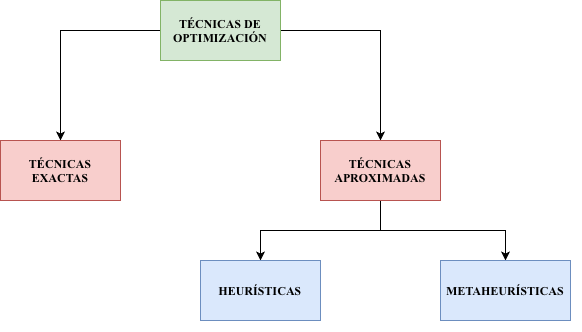
\includegraphics[width=0.85\textwidth]{./figuras/clasificacion_tecnicas_optimizacion/clasificacion_tecnicas_optimizacion.drawio.png}
% %     \caption{Clasificación general de las técnicas de optimización.}
% %     \label{fig:optimization_methods}
% % \end{figure}
% %% tecnicas exactas: garantia del optimo

% \subsection{Técnicas exactas}

% Las técnicas exactas constituyen aquellos métodos de optimización que, bajo una formulación adecuada del problema y con un presupuesto de cómputo suficiente, garantizan la obtención de la solución óptima. En este grupo se incluyen, por ejemplo, la programación lineal, la programación entera, la programación dinámica y otros procedimientos matemáticos basados en propiedades estructurales del problema.

% Su principal ventaja reside en que proporcionan garantías teóricas sobre la optimalidad de la solución obtenida. Sin embargo, esta característica suele ir acompañada de una fuerte dependencia de la formulación del problema y de un crecimiento significativo del coste computacional a medida que aumenta la complejidad del espacio de búsqueda. Por ello, cuando el problema es grande, no convexo o carece de una estructura explotable de forma directa, estas técnicas pueden resultar poco adecuadas o incluso inviables en escenarios reales.


% %% tecnicas aproximadas: sacrificio de la garantia del optimo por tiempo

% \subsection{Técnicas aproximadas}

% Aunque las técnicas exactas componen el marco de referencia desde el punto de vista teórico, en la práctica numerosos problemas de optimización deben abordarse mediante métodos aproximados capaces de proporcionar soluciones de calidad aceptable dentro de un presupuesto computacional razonable. Estas técnicas no aseguran, en general, la obtención del óptimo global, pero permiten afrontar problemas de gran escala o elevada complejidad en los que los procedimientos exactos resultan inviables por su coste o por la ausencia de una estructura suficientemente explotable \cite{boussaid2013survey}.

% El interés por este tipo de enfoques se debe a su capacidad para equilibrar calidad de solución y eficiencia temporal. Dentro de esta categoría se distinguen, de forma general, las \textbf{heurísticas} y las \textbf{metaheurísticas}, que constituyen dos de los marcos más utilizados en la optimización moderna. Aunque ambas persiguen soluciones de buena calidad en tiempos razonables, difieren en su alcance, grado de generalidad y capacidad para adaptarse a distintos problemas de optimización.

% %% heuristicas

% \subsubsection{Heurísticas}

% Generalmente, el término \textit{heurística} se utiliza para designar estrategias prácticas de resolución de problemas que permiten orientar la búsqueda de soluciones cuando no resulta viable, o no es necesario, aplicar un procedimiento exacto o exhaustivo \cite{handbookheuristics2018}. En optimización, esta idea se traduce en métodos capaces de explotar de forma eficiente la estructura del problema para obtener soluciones de calidad aceptable.

% \begin{definicion}
%     Las heurísticas son procedimientos de búsqueda orientados a obtener soluciones de buena calidad en un tiempo de cómputo reducido, sin garantizar la optimalidad de la solución obtenida.
% \end{definicion}

% Su interés radica en que permiten abordar problemas complejos en los que la resolución exacta resulta poco práctica debido al elevado coste computacional o al tamaño del espacio de búsqueda \cite{springer2024heuristics}.

% Según la forma en que generan o refinan las soluciones, las heurísticas suelen agruparse en distintas familias \cite{franca1999adaptive}. \textbf{Las heurísticas constructivas} construyen una solución desde cero, incorporando decisiones de manera progresiva hasta completar una solución factible. \textbf{Las heurísticas de mejora} parten de una solución inicial y la refinan mediante modificaciones locales orientadas a incrementar su calidad. \textbf{Las heurísticas híbridas} combinan ambos enfoques o integran estrategias adicionales de búsqueda con el objetivo de aprovechar las ventajas de cada una de ellas \cite{moreira2013hybrid}.

% %% metaheuristicas

% % - son métodos no exactos y, por lo general, no deterministas
% % - guían el proceso de búsqueda
% % - realizan una exploración eficiente del espacio de búsqueda
% % - tienen una estructura básica predefinida
% % - pueden incorporar heurísticos específicos dependientes del problema
% % - usan mecanismos para evitar regiones poco prometedoras
% % - son iterativos y disponen de criterios de parada
% % - persiguen soluciones cuasi óptimas

% % - idea: la armonización entre exploración y explotación como uno de los rasgos clave de la eficiencia de una metaheurística

% \subsubsection{Metaheurísticas}

% Las metaheurísticas constituyen una familia de métodos de optimización no exactos, diseñados para obtener soluciones de alta calidad en tiempos de cómputo razonables, especialmente en problemas complejos para los que los métodos exactos resultan inviables desde un punto de vista práctico \cite{glover1986future,talbi2009metaheuristics,boussaid2013survey}. En términos generales, se trata de procedimientos, a menudo no deterministas, concebidos para guiar de forma eficiente el proceso de búsqueda a través del espacio de soluciones \cite{talbi2009metaheuristics,luke2013essentials,marti2025fifty}.

% A diferencia de las heurísticas específicas de problema, las metaheurísticas proporcionan un marco más general de búsqueda que puede adaptarse a distintas formulaciones mediante la incorporación de operadores, reglas o mecanismos dependientes del contexto \cite{talbi2009metaheuristics,gendreau2010handbook}. Su propósito no es recorrer exhaustivamente todas las soluciones posibles, sino explorar el espacio de búsqueda de manera eficiente, favoreciendo aquellas regiones que parecen prometedoras y reduciendo el esfuerzo invertido en zonas poco rentables.

% En la mayoría de los casos, su funcionamiento se apoya en una estructura básica predefinida sobre la que se construyen mecanismos de generación, evaluación y actualización de soluciones. Este proceso se repite hasta que se satisface algún criterio de parada, como un número máximo de iteraciones, un límite temporal o una condición de convergencia \cite{luke2013essentials}. Como resultado, las metaheurísticas persiguen soluciones de calidad suficientemente alta para numerosos problemas reales, aunque sin garantizar optimalidad global \cite{glover1986future,talbi2009metaheuristics,boussaid2013survey}.

% Uno de los principios fundamentales en el diseño de metaheurísticas es el equilibrio entre exploración y explotación \cite{talbi2009metaheuristics,luke2013essentials,boussaid2013survey}. La exploración permite recorrer distintas regiones del espacio de búsqueda y reducir el riesgo de convergencia prematura, mientras que la explotación concentra el esfuerzo computacional en refinar aquellas zonas que ya han mostrado soluciones prometedoras. La capacidad para armonizar ambos comportamientos constituye uno de los elementos que más influye en la eficacia y robustez de estos métodos.


% Desde un punto de vista más abstracto, una metaheurística puede interpretarse como un esquema iterativo general compuesto por un conjunto de soluciones o estructuras de trabajo, un operador de generación de nuevas candidatas, un mecanismo de selección o reemplazo, un conjunto de variables de estado y un criterio de parada. Esta formalización, adaptada de \cite{luque2006resolucion}, permite describir bajo un mismo marco metaheurísticas de naturaleza muy distinta:
% \[
%     \mathcal{M}=\langle \Theta,\Phi,\sigma,\mu,\lambda,\Xi,\tau\rangle,
% \]
% donde \(\Theta\) es el conjunto de estructuras con las que trabaja el método, \(\Phi\) el operador que genera nuevas candidatas, \(\sigma\) la función que selecciona las estructuras que continúan en la siguiente iteración, \(\mu\) y \(\lambda\) el número de estructuras mantenidas y generadas, \(\Xi\) el conjunto de variables de estado del algoritmo y \(\tau\) el criterio de parada.

% A partir de estas características generales, las metaheurísticas pueden organizarse según distintos criterios, entre ellos el tipo de estructura sobre la que articulan la búsqueda. Esta distinción permite introducir las principales familias de métodos que se describen a continuación.

% \begin{figure}[H]
%     \centering
%     \begin{tikzpicture}[
%         node distance=0.8cm and 2.3cm,
%         every node/.style={font=\scriptsize},
%         box/.style={
%                 draw,
%                 rounded corners,
%                 align=center,
%                 minimum height=0.6cm,
%                 minimum width=2.4cm
%             },
%         rootbox/.style={
%                 box,
%                 fill=gray!15,
%                 text width=2.6cm
%             },
%         childbox/.style={
%                 box,
%                 fill=blue!8,
%                 text width=2.3cm
%             },
%         subclass/.style={
%                 box,
%                 fill=gray!3,
%                 text width=2.1cm
%             },
%         arrow/.style={
%         -{Latex[length=2mm]},
%         thick
%         }
%         ]

%         \node[rootbox] (root) {Metaheurísticas};
%         \node[childbox, below left=1.1cm and 1.5cm of root] (pop) {Basadas en\\población};
%         \node[childbox, below right=1.1cm and 0.8cm of root] (tray) {Basadas en\\trayectoria};

%         \matrix (subpops) [below=2.0cm of pop, column sep=1.8cm, row sep=0cm] {
%             \node[subclass] (enjambre) {Basadas en\\inteligencia de enjambre}; &
%             \node[subclass] (hibridas) {Híbridas};                             &
%             \node[subclass] (evolutivas) {Evolutivas};                           \\
%         };

%         \draw[arrow] (root) -- (pop);
%         \draw[arrow] (root) -- (tray);

%         \draw[arrow] (pop) -- (enjambre);
%         \draw[arrow] (pop) -- (hibridas);
%         \draw[arrow] (pop) -- (evolutivas);

%     \end{tikzpicture}
%     \caption{Clasificación general de las metaheurísticas según el tipo de estructura de búsqueda.}
%     \label{fig:clasificacion_metaheuristicas}
% \end{figure}

% \paragraph{Metaheurísticas basadas en trayectoria}

% Las metaheurísticas basadas en trayectoria se caracterizan por trabajar, en cada iteración, sobre una única solución actual o sobre un número muy reducido de soluciones estrechamente relacionadas \cite{blum2003metaheuristics,boussaid2013survey}. A partir de esa solución, el algoritmo genera nuevas candidatas mediante movimientos definidos sobre su vecindario, de modo que la búsqueda va construyendo una trayectoria a través del espacio de soluciones \cite{talbi2009metaheuristics}.

% En muchos casos, estos métodos se consideran extensiones de los procedimientos clásicos de búsqueda local. Mientras que una búsqueda local simple suele detenerse al alcanzar un óptimo local, las metaheurísticas basadas en trayectoria incorporan mecanismos adicionales para escapar de esas regiones y continuar explorando otras zonas del espacio de búsqueda \cite{gendreau2010handbook,luke2013essentials}. Entre dichos mecanismos pueden encontrarse la aceptación controlada de soluciones peores, el uso de memoria o la modificación del vecindario.

% Su principal ventaja reside en que permiten intensificar la búsqueda de manera muy eficiente alrededor de soluciones prometedoras. Sin embargo, esta misma concentración sobre una única trayectoria puede reducir la diversidad explorada y aumentar el riesgo de convergencia prematura si no se incorporan mecanismos adecuados de diversificación \cite{blum2003metaheuristics,boussaid2013survey}. Dentro de esta familia se incluyen metaheurísticas como \textit{Simulated Annealing} \cite{kirkpatrick1983optimization,vanderbilt1984monte,pedamallu2008investigating}, \textit{Tabu Search} \cite{glover1989tabu,rachid2000tabu} o \textit{Variable Neighborhood Search}. Desde la formalización abstracta introducida anteriormente, este comportamiento se corresponde típicamente con el uso de una única estructura activa por iteración, de modo que \(\mu = 1\), y con la generación de un número reducido de nuevas estructuras, por lo que \(\lambda\) suele ser pequeño.

% \paragraph{Metaheurísticas basadas en poblaciones}

% Las metaheurísticas basadas en poblaciones se caracterizan por trabajar simultáneamente con un conjunto de soluciones candidatas, en lugar de guiar la búsqueda a partir de una única solución actual \cite{blum2003metaheuristics,boussaid2013survey}. Esta característica les permite mantener activas distintas regiones del espacio de búsqueda al mismo tiempo y aprovechar la información contenida en la distribución relativa de los individuos para orientar la evolución del proceso de optimización \cite{talbi2009metaheuristics,luke2013essentials}.

% En términos generales, su funcionamiento parte de una población inicial de soluciones, a partir de la cual se generan nuevas candidatas utilizando la información disponible en los individuos ya presentes. Posteriormente, dichas soluciones se evalúan y la población se actualiza según algún criterio de selección o reemplazo \cite{talbi2009metaheuristics,boussaid2013survey}. El intercambio de información entre soluciones puede modelarse de distintas maneras, como la recombinación entre individuos, el uso de diferencias entre soluciones o la atracción hacia posiciones prometedoras.

% Una de las principales ventajas de esta familia es su elevada capacidad exploratoria. Al mantener múltiples soluciones simultáneamente, las metaheurísticas poblacionales pueden muestrear distintas zonas del espacio de búsqueda, identificar regiones prometedoras y reducir el riesgo de convergencia prematura asociado a la concentración temprana en una sola trayectoria \cite{blum2003metaheuristics,boussaid2013survey,omidvar2022review}. No obstante, esta ventaja suele ir acompañada de un mayor coste computacional por iteración, ya que en cada ciclo deben evaluarse varias soluciones candidatas. Esta observación resulta especialmente relevante en problemas con funciones objetivo costosas, donde el uso de grandes poblaciones puede hacer necesario recurrir a estrategias de aceleración, paralelización o modelado \textit{surrogate} \cite{omidvar2022review}.

% Desde la formalización abstracta introducida anteriormente, las metaheurísticas basadas en poblaciones se caracterizan por operar con varias estructuras activas en cada iteración, por lo que \(\mu > 1\). Del mismo modo, el número de nuevas estructuras generadas en cada ciclo también suele ser superior al de los métodos basados en trayectoria, de manera que \(\lambda > 1\).

% \subparagraph{Metaheurísticas poblacionales basadas en inteligencia de enjambre}

% Las metaheurísticas basadas en inteligencia de enjambre modelan comportamientos colectivos descentralizados, en los que múltiples agentes interactúan entre sí y con el entorno para orientar la búsqueda. En esta familia se sitúan, entre otros, \textit{Particle Swarm Optimization} \cite{kennedy1995pso} o \textit{Ant Colony Optimization} \cite{socha2008aco}.

% \subparagraph{Metaheurísticas poblacionales híbridas}

% Las metaheurísticas híbridas poblacionales combinan mecanismos de búsqueda poblacional con procedimientos adicionales de intensificación, como búsqueda local o estrategias meméticas, con el objetivo de combinar exploración global y refinamiento local \cite{lozano2004memetic,ong2004metalamarckian,renders1996hybrid,hart1994adaptive}. Dentro de este panorama también pueden situarse enfoques basados en modelado probabilístico, como los \textit{Estimation of Distribution Algorithms} \cite{ahn2008eda}.

% \subparagraph{Metaheurísticas poblacionales evolutivas}

% Los algoritmos evolutivos (EA) constituyen una familia de metaheurísticas poblacionales inspiradas en los mecanismos de adaptación y evolución observados en la naturaleza. De forma general, operan sobre una población de individuos que representan soluciones candidatas al problema. A lo largo del proceso de búsqueda, dicha población evoluciona mediante operadores de selección, variación y reemplazo \cite{holland1975adaptation,mitchell1998introduction,reeves2003genetic,affenzeller2009genetic}. Cada individuo recibe una valoración cuantitativa a través de una función de aptitud o \textit{fitness}, que mide la calidad de la solución representada y guía el proceso de búsqueda.

% De forma abstracta, la dinámica de un algoritmo evolutivo puede resumirse en el Algoritmo~\ref{alg:ea_general}. En primer lugar, se genera una población inicial y se evalúa su calidad. A continuación, mientras no se satisfaga el criterio de parada, se seleccionan progenitores, se aplican operadores de recombinación y mutación para generar descendencia, se evalúan los nuevos individuos y se actualiza la población mediante algún mecanismo de reemplazo. El proceso iterativo finaliza devolviendo la mejor solución encontrada.

% \begin{algorithm}[H]
%     \caption{Esquema general de un algoritmo evolutivo}
%     \label{alg:ea_general}
%     \begin{algorithmic}[1]
%         \State $P \gets \textsc{GenerarPoblacionInicial}()$
%         \State $\textsc{Evaluar}(P)$
%         \While{no se cumpla el criterio de parada}
%         \State $P' \gets \textsc{SeleccionarPadres}(P)$
%         \State $P' \gets \textsc{Recombinar}(P')$
%         \State $P' \gets \textsc{Mutar}(P')$
%         \State $\textsc{Evaluar}(P')$
%         \State $P \gets \textsc{SeleccionarNuevaPoblacion}(P, P')$
%         \EndWhile
%         \State \Return mejor solución encontrada
%     \end{algorithmic}
% \end{algorithm}

% Dentro de esta familia se incluyen distintas líneas metodológicas, entre ellas los algoritmos genéticos, las estrategias evolutivas y métodos posteriores como \textit{Differential Evolution}, que comparten el enfoque poblacional y evolutivo, aunque difieren en la forma en que generan nueva descendencia y en los operadores que emplean.

% %% no muy largo

% % por que evaluar puede ser el cuello de botella
% % por que esto limita la aplicación prácitca de metaheurísticas
% % necesidad de reducir el número de evaluaciones necesarias para alcanzar soluciones de calidad
% % técnicas surrogate como una posible solución a este problema

% %% El concepto clave: Introduce el término "Presupuesto Computacional" (Computational Budget). Explica que, en el mundo real, no tienes "infinitas evaluaciones", sino quizás solo 500 o 1000 porque cada una tarda 10 minutos.
% %% Consecuencia: Si el presupuesto es bajo, la metaheurística no puede converger. Aquí es donde los modelos surrogate salvan el día.

% \section{Diversidad, estancamiento y convergencia prematura}
% \label{sec:diversidad_estancamiento}

% Durante el proceso iterativo de una metaheurística poblacional, la búsqueda suele alternar entre fases de exploración global y de intensificación sobre regiones prometedoras del espacio de soluciones. Esta dinámica resulta esencial, ya que permite explorar distintas zonas del espacio de búsqueda y refinar progresivamente aquellas que han mostrado mejores resultados. No obstante, también puede conducir a una reducción progresiva de la diversidad poblacional, especialmente cuando los individuos comienzan a concentrarse en torno a un conjunto reducido de soluciones de alta calidad \cite{talbi2009metaheuristics,boussaid2013survey,squillero2016divergence}.

% \begin{definicion}
%     La \textbf{diversidad poblacional} hace referencia a la variedad y heterogeneidad de las soluciones candidatas presentes en la población de una metaheurística. Mantener una diversidad adecuada es crucial para evitar el estancamiento y favorecer la exploración efectiva del espacio de búsqueda.
% \end{definicion}

% En este contexto, la diversidad es un elemento fundamental para el correcto funcionamiento de las metaheurísticas basadas en población, especialmente en problemas con paisajes de búsqueda complejos, multimodales o engañosos. Una diversidad moderada-alta favorece la exploración de múltiples regiones del espacio de soluciones, reduce la probabilidad de caer rápidamente en zonas subóptimas y mantiene la capacidad del algoritmo para generar nuevas soluciones suficientemente distintas entre sí. Por el contrario, cuando la diversidad disminuye drásticamente, la población tiende a volverse cada vez más homogénea, lo que limita la eficacia de los operadores de variación y reduce la posibilidad de descubrir regiones no exploradas previamente, dando lugar al \textbf{estancamiento} \cite{omidvar2022review,squillero2016divergence,sudholt2018benefits}.

% En términos generales, puede decirse que un algoritmo entra en \textbf{estancamiento} cuando, aun continuando con su ejecución, deja de producir mejoras significativas en la calidad de las soluciones durante un número prolongado de iteraciones o evaluaciones. Este comportamiento suele aparecer cuando la población queda atrapada en una región cuya explotación adicional apenas genera progreso. Si esta concentración ocurre demasiado pronto, o incluso en torno a un óptimo local, la explotación pasa a dominar de forma excesiva sobre la exploración y la diversidad poblacional se colapsa antes de que el algoritmo haya revisado de forma suficientemente amplia otras zonas potencialmente prometedoras. En consecuencia, esta situación de \textbf{convergencia prematura} puede interpretarse como uno de los principales mecanismos que conducen al estancamiento en metaheurísticas poblacionales \cite{pandey2014premature,squillero2016divergence,sudholt2018benefits}.

% En el contexto de este trabajo, estos conceptos son muy importantes debido al uso posterior de técnicas \textit{surrogate}. Cuando la población ha convergido de forma excesiva y los individuos se vuelven prácticamente indistinguibles entre sí, la variabilidad estructural de las muestras se reduce notablemente y la capacidad del modelo para discriminar entre soluciones pierde utilidad práctica. En estas condiciones, tanto la predicción como el ranking entre candidatos tienden a aportar menos información relevante para orientar la búsqueda.

% % Para mitigar este tipo de situaciones, en la literatura resulta habitual incorporar \textbf{mecanismos de reinicio} orientados a reactivar la exploración cuando el proceso de búsqueda muestra señales claras de pérdida de diversidad o ausencia prolongada de mejora \cite{fukunaga1998restart,lozano2008replacement,luna2025elitist}. La idea general consiste en regenerar total o parcialmente la población con el fin de desplazar la búsqueda hacia nuevas regiones del espacio de soluciones. En este contexto, un \textit{reinicio aleatorio} o \textit{reinicio desde cero} regenera completamente la población, mientras que un \textit{reinicio elitista} preserva una parte de la información previamente adquirida. No obstante, un reinicio completo puede conllevar la pérdida de información valiosa acumulada durante la ejecución, especialmente cuando el algoritmo ya ha identificado soluciones de alta calidad. Por ello, en este y en muchos otros contextos resulta preferible optar por un enfoque de \textbf{reinicio elitista}, que no elimina toda la información previa, sino que preserva uno o varios de los mejores individuos encontrados hasta ese momento y regenera el resto, buscando combinar recuperación de diversidad y mantenimiento del progreso acumulado. En consecuencia, el reinicio elitista puede interpretarse como un mecanismo de control de la dinámica poblacional que busca restaurar la capacidad exploratoria del algoritmo sin renunciar completamente a la explotación de la información previamente adquirida \cite{fukunaga1998restart,lozano2008replacement,luna2025elitist}. Sobre esta base conceptual, en la Sección~\ref{subsec:metodologia_reinicio} se especifica el criterio de reinicio elitista concreto adoptado en este trabajo.

% Para mitigar este tipo de situaciones, en la literatura se utilizan \textbf{mecanismos de reinicio} encargados de reactivar la exploración cuando el proceso de búsqueda muestra señales claras de pérdida de diversidad o ausencia prolongada de mejora \cite{fukunaga1998restart,lozano2008replacement,luna2025elitist}. La idea general consiste en regenerar total o parcialmente la población con el fin de desplazar la búsqueda hacia nuevas regiones del espacio de soluciones. En este contexto, un \textit{reinicio aleatorio} o \textit{reinicio desde cero} regenera completamente la población, mientras que un \textit{reinicio elitista} preserva una parte de la información previamente adquirida.

% \section{Técnicas surrogadas}

% %% Riesgos: No olvides mencionar el error de aproximación. Si el modelo es malo, guiará a la metaheurística hacia un "óptimo falso". Esto justifica por qué necesitamos la hibridación online (para re-entrenar el modelo).

% % definicion 
% % idea general
% % familias de modelos
% % modelos principales
% % ventajas y riesgos 

% \begin{definicion}
%     Sea \(f:\mathcal{X}\rightarrow\mathbb{R}\) una función objetivo costosa de evaluar. Un \textit{surrogate model} es una función aproximada \(\hat{f}:\mathcal{X}\rightarrow\mathbb{R}\), construida a partir de un conjunto finito de muestras
%     \[
%         \mathcal{D}=\{(\mathbf{x}_i,f(\mathbf{x}_i))\}_{i=1}^{n},
%     \]
%     con el objetivo de proporcionar información útil sobre el comportamiento de \(f\) de forma computacionalmente más eficiente. En muchos casos, esta información se materializa como una función aproximada \(\hat{f}:\mathcal{X}\rightarrow\mathbb{R}\), aunque también puede adoptar otras formas orientadas a comparar, clasificar o priorizar soluciones.
% \end{definicion}

% En problemas de optimización con funciones costosas, como los basados en simulación, la evaluación repetida de la función objetivo puede suponer un coste computacional elevado o incluso prohibitivo \cite{queipo2005surrogate,forrester2009recent}. En este contexto, las técnicas surrogadas permiten sustituir parcial o temporalmente la función real por una aproximación de menor complejidad, de modo que el proceso de búsqueda pueda orientarse utilizando una representación más barata de evaluar.

% Aunque los modelos surrogados suelen plantearse como aproximaciones de la función objetivo, su utilidad en optimización no se limita necesariamente a predecir con precisión el valor numérico de \(f\). En muchos casos, resulta suficiente con que proporcionen información útil para orientar la búsqueda, por ejemplo preservando el orden relativo entre soluciones, discriminando entre candidatas prometedoras y no prometedoras o apoyando decisiones de selección sin necesidad de reproducir exactamente la función original \cite{jin2011surrogate,tong2021surrogate}.

% El interés principal de estos métodos es que permiten reutilizar la información obtenida en evaluaciones previas para guiar la búsqueda hacia regiones realmente prometedoras, manteniendo una representación útil del comportamiento del problema con un coste de evaluación mucho menor \cite{queipo2005surrogate,forrester2009recent,jin2011surrogate}. Esto resulta especialmente útil cuando cada evaluación implica ejecutar un simulador, resolver un problema físico o analizar un modelo complejo. Además, su flexibilidad hace posible adaptarlos a distintos tipos de formulaciones, desde enfoques regresivos orientados a aproximar valores hasta estrategias basadas en clasificación o en comparaciones relativas entre soluciones.

% No obstante, su utilización también plantea limitaciones importantes. Si el surrogate no está bien ajustado, puede inducir al algoritmo de optimización a explorar regiones poco prometedoras, establecer un orden incorrecto entre soluciones o descartar candidatas que en realidad serían buenas. Asimismo, muchos modelos presentan dificultades para generalizar fuera de las zonas en las que han sido entrenados, lo que restringe su utilidad en espacios de búsqueda muy amplios o con una estructura altamente no lineal \cite{forrester2009recent,bhosekar2018advances}. Por ello, la eficacia de estos métodos depende tanto de la calidad del modelo construido como del tipo de información que se pretenda extraer de él y del modo en que se integre dentro del proceso de optimización.

% En el contexto de la optimización, y en particular dentro de algoritmos evolutivos y metaheurísticos, los surrogates pueden desempeñar papeles muy distintos según el modo en que se utilicen y el tipo de información que proporcionen al algoritmo de búsqueda \cite{jin2011surrogate,tong2021surrogate}. Por ello, antes de describir los modelos utilizados comúnmente, resulta conveniente introducir una visión general de las principales taxonomías utilizadas en la literatura para clasificar este tipo de técnicas.

% \subsection{Taxonomía general de las técnicas surrogadas}

% La literatura especializada no clasifica los modelos surrogados siguiendo un único criterio, sino que suele hacerlo desde perspectivas complementarias. En algunos casos, la clasificación se centra en el papel funcional que desempeña el surrogate dentro del proceso de optimización, mientras que en otros se corresponde con el tipo de información que el modelo es capaz de predecir sobre las soluciones candidatas. Ambas perspectivas son útiles, ya que permiten entender tanto cómo se utiliza el surrogate como qué tipo de apoyo proporciona al algoritmo de búsqueda.

% \subsubsection{Integración del surrogate en la optimización}

% Una de las formas más extendidas de clasificar las técnicas surrogadas, propuesta en \cite{bliek2022sustainableSBO}, consiste en atender al modo en que el modelo sustituto se integra dentro del proceso de optimización. Desde esta perspectiva, el surrogate no se distingue únicamente por su naturaleza estadística o de aprendizaje, sino por el papel funcional que desempeña respecto de la función objetivo original y del algoritmo de búsqueda. Así, pueden distinguirse enfoques en los que el surrogate se actualiza de forma iterativa durante la optimización, otros en los que sustituye completamente a la función costosa una vez entrenado, y también estrategias en las que se reutiliza información de procesos previos o se combina con otras formas de intervención o decisión.

% Esta clasificación resulta especialmente útil porque permite diferenciar no solo cómo se construye el surrogate, sino también cuándo se consulta, qué tipo de interacción mantiene con la función real y qué grado de acoplamiento presenta con el optimizador. En consecuencia, ofrece una visión más operativa del uso de modelos sustitutos en optimización que otras taxonomías centradas exclusivamente en el tipo de modelo de regresión o clasificación empleado.

% \paragraph{Sequential Model-Based Optimization (SMBO)}

% El enfoque \textit{Sequential Model-Based Optimization} se caracteriza por la alternancia iterativa entre el surrogate y la función objetivo costosa. En una primera fase se evalúa un conjunto inicial de soluciones sobre la función real con el fin de construir un conjunto de entrenamiento. A partir de esos datos se ajusta un modelo sustituto, que posteriormente se utiliza para proponer nuevas soluciones prometedoras. Dichas soluciones son evaluadas de nuevo en la función real y la información obtenida se incorpora al conjunto de entrenamiento para actualizar el surrogate.

% La característica distintiva de este esquema es que el modelo no sustituye de forma definitiva a la función costosa, sino que se refina progresivamente a medida que avanza la búsqueda. De este modo, el surrogate actúa como un mecanismo auxiliar que orienta la exploración y reduce el número de evaluaciones reales necesarias, por lo que este tipo de métodos suele identificarse con estrategias \textit{online}.

% \begin{figure}[H]
%     \centering
%     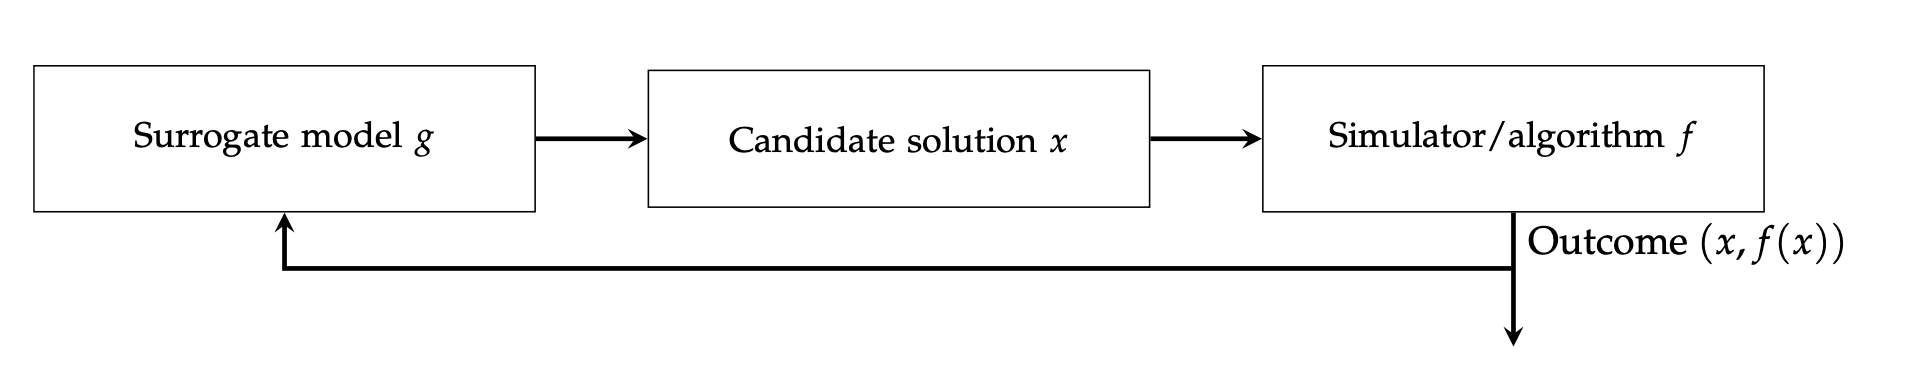
\includegraphics[width=0.95\textwidth]{./figuras/clasificacion_surrogates/smbo.png}
%     \caption{Framework simplificado de un algoritmo SMBO típico obtenido de \cite{bliek2022sustainableSBO}.}
%     \label{fig:smbo}
% \end{figure}

% La Figura~\ref{fig:smbo} muestra este ciclo de realimentación continua entre surrogate, optimización y evaluación real, donde cada nueva evaluación contribuye a mejorar la calidad del modelo.

% \paragraph{Predict-then-Optimise (PtO)}

% En el enfoque \textit{Predict-then-Optimise}, el surrogate se entrena previamente a partir de un conjunto de muestras evaluadas sobre la función real y, una vez construido, pasa a sustituir completamente a la función costosa durante la fase de optimización. En este caso, el algoritmo de búsqueda opera directamente sobre el modelo sustituto, como si éste fuese la verdadera función objetivo.

% La principal ventaja de este esquema radica en que, tras el entrenamiento inicial, la búsqueda puede desarrollarse sin recurrir continuamente a la función real, lo que reduce de forma drástica el coste computacional. Sin embargo, la calidad del resultado final depende en gran medida de la fidelidad global del surrogate, ya que cualquier sesgo o error acumulado en el modelo afectará directamente a la solución obtenida. Por este motivo, este enfoque suele asociarse a estrategias \textit{offline}.

% \begin{figure}[H]
%     \centering
%     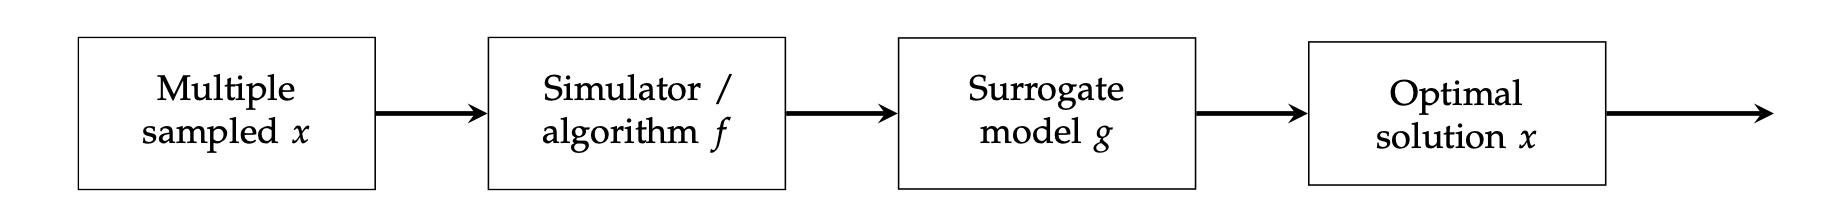
\includegraphics[width=1.00\textwidth]{./figuras/clasificacion_surrogates/pto.png}
%     \caption{Framework de Predict-then-Optimise (PtO) típico obtenido de \cite{bliek2022sustainableSBO}.}
%     \label{fig:pto}
% \end{figure}

% La Figura~\ref{fig:pto} ilustra esta separación entre la fase de construcción del surrogate y la fase posterior de optimización, sin actualización iterativa del modelo durante la búsqueda.

% \paragraph{Otras formas de integración}

% Además de los dos esquemas anteriores, la literatura recoge otras formas de integración del surrogate dentro del proceso de optimización \cite{bliek2022sustainableSBO}. El enfoque \textit{Optimise-then-Predict} (OtP) se orienta al aprovechamiento de información obtenida en optimizaciones previas para construir modelos reutilizables en problemas futuros similares. Por su parte, \textit{Predict-then-Interact} (PtI) emplea el surrogate como herramienta de apoyo a la intervención humana, de modo que el modelo no guía únicamente una optimización automática, sino también la toma de decisiones por parte del usuario.

% Asimismo, en problemas jerárquicos o anidados, los surrogates pueden utilizarse para aproximar subproblemas internos, como ocurre en ciertos esquemas de optimización bi-nivel. También existen enfoques en los que la propia construcción del surrogate se automatiza mediante procedimientos de \textit{Automated Machine Learning} o en los que se combinan varios modos de uso dentro de un mismo método, dando lugar a estrategias mixtas. Aunque estas variantes amplían el panorama de integración posible, en este trabajo resultan especialmente relevantes los esquemas SMBO y PtO, por su conexión directa con los enfoques \textit{online} y \textit{offline} considerados posteriormente.

% \paragraph{Optimise-then-Predict (OtP)}

% El enfoque \textit{Optimise-then-Predict} invierte parcialmente la lógica anterior. En este caso, primero se ejecutan procesos de optimización sobre la función costosa y, una vez obtenida información suficiente de esas ejecuciones, se construye un surrogate que permita reutilizar el conocimiento adquirido en problemas futuros similares. El modelo no se emplea necesariamente para guiar la búsqueda actual, sino como una forma de transferir experiencia de optimizaciones previas.

% Se trata, por tanto, de una categoría más amplia y menos homogénea que las anteriores, ya que incluye métodos orientados al ahorro de evaluaciones en escenarios repetitivos o familias de problemas emparentadas. Su interés reside en el aprovechamiento de información acumulada, de forma que el coste de optimización de instancias futuras pueda reducirse gracias a la experiencia acumulada.

% \begin{figure}[H]
%     \centering
%     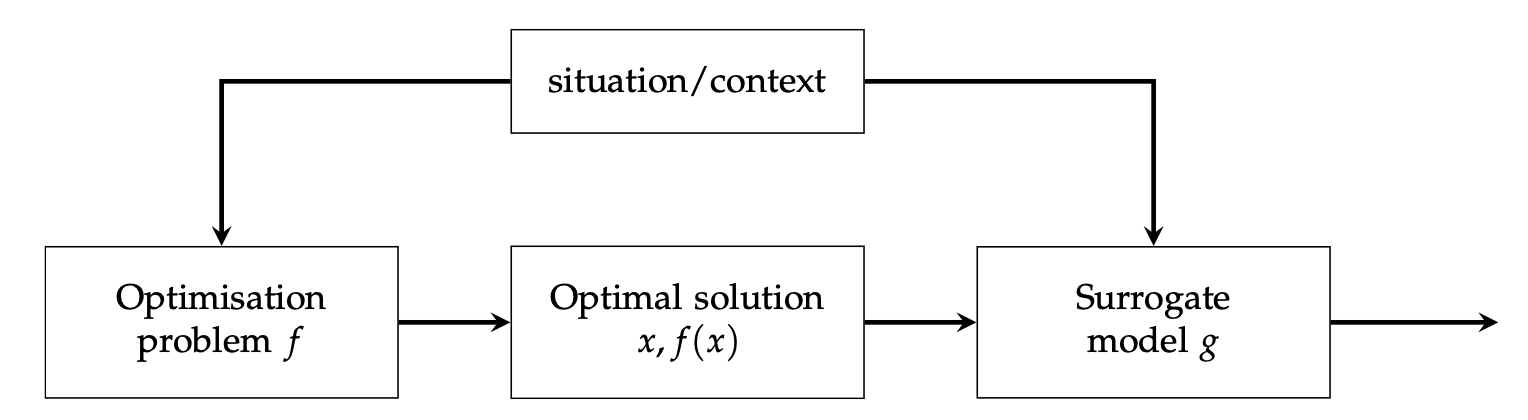
\includegraphics[width=0.95\textwidth]{./figuras/clasificacion_surrogates/otp.png}
%     \caption{Framework de Optimise-then-Predict (OtP) típico obtenido de \cite{bliek2022sustainableSBO}.}
%     \label{fig:otp}
% \end{figure}

% La Figura~\ref{fig:otp} refleja esta inversión del flujo habitual, en la que la optimización precede a la construcción del surrogate y el modelo se utiliza principalmente como mecanismo de reutilización de conocimiento.

% \paragraph{Predict-then-Interact (PtI)}

% El enfoque \textit{Predict-then-Interact} comparte con PtO la idea de construir un surrogate antes de la toma de decisiones, pero en este caso el modelo no es optimizado automáticamente por un algoritmo, sino utilizado como apoyo para la intervención humana. El usuario o experto del dominio inspecciona las predicciones del surrogate e interactúa con ellas para dirigir el proceso hacia soluciones consideradas prometedoras.

% Este esquema resulta especialmente relevante en contextos donde la experiencia humana, la interpretación del problema o la subjetividad del criterio de evaluación desempeñan un papel importante. A diferencia de los enfoques puramente automáticos, aquí el surrogate funciona como herramienta de asistencia a la decisión y no exclusivamente como sustituto computacional de la función objetivo.

% \begin{figure}[H]
%     \centering
%     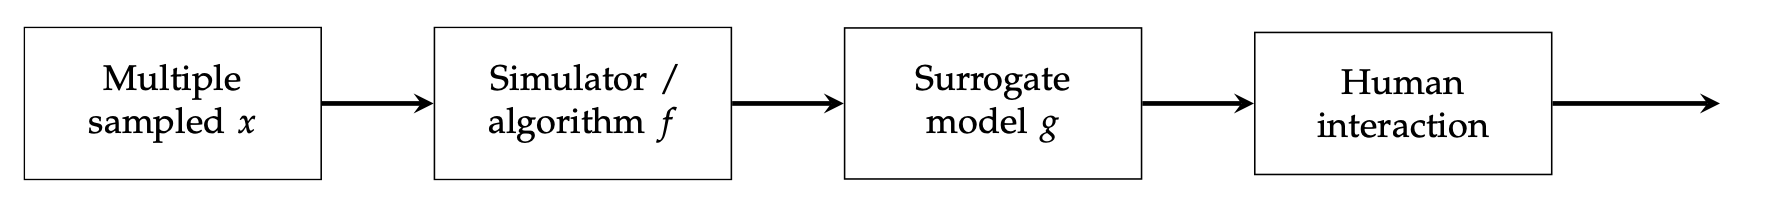
\includegraphics[width=0.95\textwidth]{./figuras/clasificacion_surrogates/pti.png}
%     \caption{Framework de Predict-then-Interact (PtI) típico obtenido de \cite{bliek2022sustainableSBO}.}
%     \label{fig:pti}
% \end{figure}

% La Figura~\ref{fig:pti} pone de manifiesto que el elemento diferencial de este enfoque no es la optimización automática del modelo, sino la interacción del usuario con las predicciones generadas para orientar el proceso de búsqueda.

% \paragraph{Bi-level Optimization (BlO)}

% La \textit{Bi-level Optimization} agrupa aquellos enfoques en los que el problema de optimización está estructurado en dos niveles jerárquicos, de modo que la solución del nivel inferior depende de las decisiones adoptadas en el nivel superior. En este contexto, el surrogate suele emplearse para aproximar el problema interno, reduciendo así el coste de resolver repetidamente dicho subproblema durante la búsqueda en el nivel externo.

% La utilidad del surrogate en este caso no proviene tanto de reemplazar la función objetivo completa, sino de simplificar una de las capas del problema.

% Esto hace que su papel sea especialmente relevante en escenarios donde la optimización anidada resulta prohibitiva desde el punto de vista computacional.

% \paragraph{Automated Machine Learning (AutoML)}

% La categoría \textit{Automated Machine Learning} incorpora los casos en los que el uso del surrogate se integra dentro de procedimientos automáticos de selección, ajuste o combinación de modelos y configuraciones. En este marco, el propio proceso de construir el surrogate puede ser objeto de optimización, de modo que la elección del modelo, sus hiperparámetros o incluso la estrategia de uso del surrogate se decidan de forma automática.

% Aunque esta categoría suele quedar parcialmente fuera del núcleo clásico de la optimización surrogate, resulta conceptualmente relevante porque enfatiza la automatización del diseño del modelo sustituto y de su integración con el algoritmo de búsqueda.

% \paragraph{Mixed Surrogate-Based}

% La categoría \textit{Mixed Surrogate-Based} engloba aquellas estrategias híbridas en las que se combinan varios de los enfoques anteriores o en las que el surrogate desempeña múltiples funciones dentro del mismo procedimiento. Por ejemplo, pueden coexistir fases \textit{online} y \textit{offline}, mecanismos de actualización adaptativa del surrogate, combinación de varios modelos o integración simultánea con distintas estrategias de decisión.

% Este tipo de enfoques mixtos refleja la tendencia reciente a diseñar procedimientos más flexibles y adaptativos, en los que el surrogate no se concibe como un componente fijo, sino como una herramienta que puede cambiar de papel según la fase de la optimización, la información disponible o el comportamiento observado durante la búsqueda. En esta línea, la combinación explícita de varios modelos surrogate ha sido propuesta en la literatura como una vía para mejorar la robustez de la aproximación frente a la dependencia de un único modelo \cite{goel2007ensemble}.

% \subsubsection{Tipo de predicción}

% Otra forma útil de clasificar los modelos surrogados se basa en la naturaleza de la información que proporcionan sobre las soluciones candidatas. Desde esta perspectiva, la diferencia fundamental no reside en el algoritmo de aprendizaje utilizado, sino en si el surrogate intenta aproximar directamente el valor numérico de la función objetivo o si, por el contrario, modela únicamente relaciones relativas entre soluciones, como su orden, preferencia o pertenencia a una determinada clase \cite{tong2021surrogate}.

% Esta distinción es crucial en optimización con surrogates, ya que condiciona tanto el diseño del modelo como su integración dentro del algoritmo evolutivo. En algunos problemas interesa aproximar con la mayor fidelidad posible la función objetivo, mientras que en otros basta con determinar qué soluciones son mejores que otras sin necesidad de conocer su fitness exacto. En este contexto, la literatura distingue entre modelos de \textit{absolute fitness} y modelos de \textit{relative fitness}, cada uno con subcategorías específicas \cite{tong2021surrogate}.

% \begin{figure}[H]
%     \centering
%     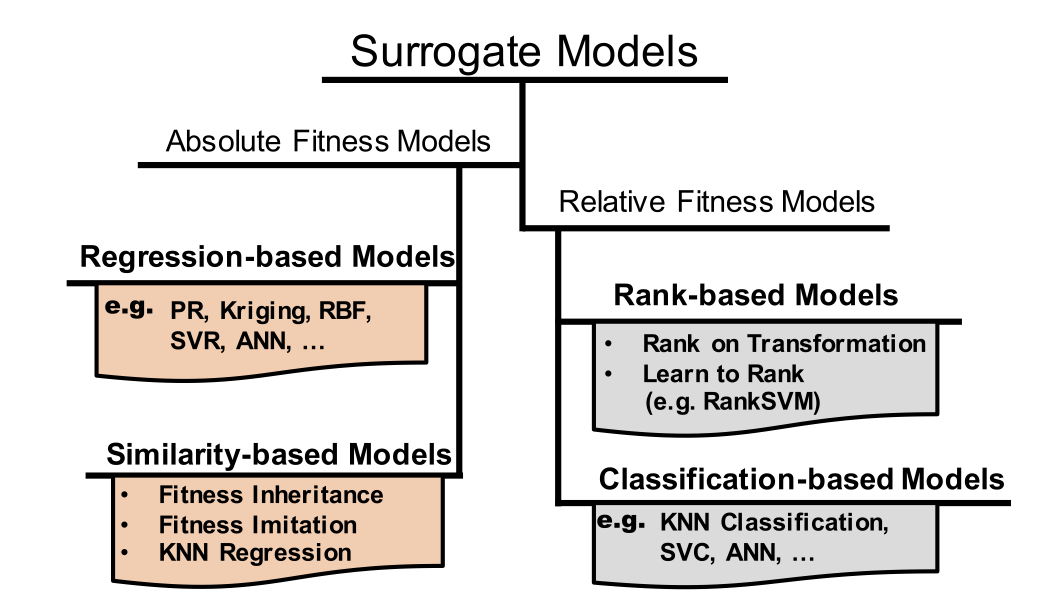
\includegraphics[width=0.7\textwidth]{./figuras/clasificacion_surrogates/clasificacion_sgs.png}
%     \caption{Clasificación de las técnicas surrogadas según el tipo de predicción, adaptada de \cite{tong2021surrogate}.}
%     \label{fig:clasificacion_sgs}
% \end{figure}

% \medskip
% \noindent\textbf{\large Modelos de fitness absoluto}\par
% \smallskip

% Los \textit{absolute fitness models} tratan de aproximar directamente el valor de la función objetivo de una solución candidata. Su propósito consiste en construir una función sustituta \(\hat{F}\) que reproduzca, con la mayor fidelidad posible, la relación entre el vector de decisión \(\mathbf{x}\) y su fitness real \(F(\mathbf{x})\). Se trata de la formulación más clásica en optimización basada en surrogates, ya que permite reemplazar evaluaciones costosas por predicciones numéricas explícitas del fitness.

% \smallskip
% \noindent\textbf{Modelos basados en regresión}\par
% \smallskip

% Dentro de los modelos de fitness absoluto, los \textit{regression-based models} constituyen la familia más común. Su objetivo es ajustar un modelo que aproxime el mapeo entre las variables de decisión y el valor escalar de fitness. Dado un conjunto de entrenamiento de la forma
% \[
%     D=\{(\mathbf{x}_1,y_1),(\mathbf{x}_2,y_2),\dots,(\mathbf{x}_n,y_n)\},
% \]
% donde \(y_i=F(\mathbf{x}_i)\), el surrogate se construye buscando minimizar la relación entre los valores reales y las predicciones del modelo.

% En esta categoría se incluyen, por ejemplo, la regresión polinómica, Kriging, las funciones de base radial, redes neuronales o métodos de ensamblado adaptados a regresión. Su ventaja principal es que proporcionan una estimación explícita del fitness, lo que permite utilizarlos directamente en operadores de selección, reemplazo o preevaluación dentro de algoritmos evolutivos.

% \smallskip
% \noindent\textbf{Modelos basados en similitud}\par
% \smallskip

% Los \textit{similarity-based models} también pertenecen a la categoría de fitness absoluto, pero estiman el fitness de nuevas soluciones a partir de su cercanía o relación con muestras previamente evaluadas. En lugar de aprender una función global explícita, estos enfoques basan la predicción en relaciones locales dentro del espacio de búsqueda. Su comportamiento depende, en gran medida, de la métrica de distancia empleada y de la distribución de las muestras disponibles.

% \medskip
% \noindent\textbf{\large Modelos de fitness relativo}\par
% \smallskip

% Los \textit{relative fitness models} no intentan predecir directamente el valor numérico de la función objetivo, sino estimar información relativa entre soluciones candidatas. En lugar de responder a la pregunta “¿cuál es el fitness de esta solución?”, estos modelos tratan de responder cuestiones como “¿qué solución es mejor?”, “¿cuál ocupa una posición más alta en el ranking?” o “¿a qué categoría de calidad pertenece esta muestra?”. Este enfoque resulta especialmente interesante en contextos donde el valor exacto del fitness es difícil de estimar o menos relevante que la capacidad de discriminar correctamente entre candidatos.

% \smallskip
% \noindent\textbf{Modelos basados en ranking}\par
% \smallskip

% Los \textit{rank-based models} constituyen una primera subcategoría dentro de los modelos de fitness relativo. Su objetivo es estimar el orden relativo de las soluciones, es decir, aprender qué candidatos deberían situarse por delante de otros en términos de calidad. En optimización evolutiva, esta aproximación puede resultar suficiente cuando el algoritmo necesita principalmente información de preferencia para seleccionar, reemplazar o priorizar individuos. Su interés radica en que, en muchos problemas, preservar correctamente el orden relativo entre soluciones puede ser más importante, y también menos costoso que ajustar con precisión sus valores absolutos \cite{yuxue2024effective}.

% \smallskip
% \noindent\textbf{Modelos basados en clasificación}\par
% \smallskip

% La segunda subcategoría de los modelos de fitness relativo es la formada por los \textit{classification-based models}. En este caso, el surrogate asigna las soluciones a distintas clases o categorías, por ejemplo distinguiendo entre individuos prometedores y no prometedores, o separando regiones de alta y baja calidad en el espacio de búsqueda. Este enfoque puede ser muy útil cuando el objetivo principal es filtrar candidatos \cite{jinglu2022classification,lin2023classification}, concentrar evaluaciones costosas en soluciones de interés o guiar el proceso de exploración.

% \section{Hibridación entre metaheurísticas y modelos surrogate}

% integración offline/online
% papel del surrogate en la busqueda de soluciones
% enfoques de hibridación offline
% ....
% enfoques de hibridación online
% surrogate como filtro de soluciones candidatas
% surrogate como guía para la generación de nuevas soluciones
% surrogate como mecanismo de selección entre operadores o estrategias de búsqueda

%%%%%

% probability-based-strategy:  probabilidad aleatoria de no usar el surrogate
% baseline strategy: se usa el surrogate en todas las evaluaciones - SIEMPRE
% candidate diversity strategy: 
% quality distance strategy: diferencia entre el fitness estimado del challenger y el fitness del challenged


% Una vez analizados los pilares conceptuales de la optimización y el modelado predictivo, se evidencia que la hibridación de algoritmos evolutivos junto con modelos de aprendizaje automático y técnicas subrogadas ofrece un marco robusto para mitigar el coste computacional. En los capítulos sucesivos se abordará cómo la literatura científica reciente ha combinado ambas disciplinas (Capítulo 4) y se detallarán las arquitecturas algorítmicas específicas, el banco de problemas CEC2017 y los modelos de regresión seleccionados como referencia para la fase experimental de este trabajo (Capítulo 5).
